


\begin{abstract}[\hspace*{-10pt}]
    This chapter draws mainly on the published works: \fullcite{van_biesbroeck_reference_2024}%\\  % Ce chapitre reprend principalement les travaux publiés dans: 
    %and: \fullcite{van_biesbroeck_influence_2023}
\end{abstract}

\begin{abstract}
    For many structures of interest, estimating seismic fragility curves is a daunting task because of the limited amount of data available, and the limited amount of information they contain
    (such as binary data, i.e. only describing the structure as being in a failure or non-failure state).
    In such a context, a probit-lognormal modeling of the fragility curve is prominent, 
    and among various methods that exist to estimate the parameters of the model, the Bayesian inference became popular in the literature. However, the trustworthiness of the latter relies on the prior selection, jeopardizing the approach if the selection is motivated by subjective considerations.
    This chapter proposes a comprehensive objective Bayesian estimation of seismic fragility curves, implementing the Jeffreys prior for the probit-lognormal model.
    This prior is completely studied along with the decay rates of the likelihood to ensure the validity of our methodology.
    %
    %
    %The posterior distribution is proven to be proper (i.e., it integrates to unity) with the Jeffreys prior but improper with some traditional priors found in the literature. With the Jeffreys prior, the posterior distribution is also shown to vanish at the boundaries of the parameters' domain, which means that sampling the posterior distribution of the parameters does not result in anomalously small or large values.
    It is also implemented on the three case studies detailed in   \cref{chap:frags-intro}. 
    % It is also implemented on three different case studies, including industrial examples. %--- to illustrate the theoretical 
    Our theoretical and practical results show that the Jeffreys prior leads to more robust and efficient fragility curves estimates in comparison with other methods of the literature. 
%
 %   Therefore, the use of the Jeffreys prior does not result in degenerate fragility curves such as unit-step functions, and leads to more robust credibility intervals. The numerical results obtained from two different case studies---including an industrial example---illustrate the theoretical predictions.
    %For estimating seimsic fragility curves wh
    %Seismic fragility curves 
\end{abstract}


\minitoc

\section{Introduction}


Seismic fragility curves are key quantities of interest of the seismic probabilistic risk assessment (SPRA) framework.
They are defined as the probability of failure of a mechanical system conditionally to a scalar value that is derived from a seismic signal, coined intensity measure (IM).
A detailed review of those curves and of the methods that exist to estimate them is proposed in   \cref{chap:frags-intro}.

Although various data sources can be exploited to evaluate such curves, most of them  suffer from their scarcity,
complicating the uncertainty quantification in the estimates.
Moreover, we focus in this work on cases where the dataset contains information of the mechanical system's response under seismic excitation that is limited to binary outcome, i.e. failure or non-failure.
In this sense, this work will mainly address equipment problems for which only binary results of seismic qualification tests (e.g., tests of electrical relays, etc.) or empirical data such as presented in \cite{straub_improved_2008} are available. However, the methodology developed here could perfectly be applied to simulation-based approaches as well.


%we focus in this work on cases where 
%In this chapter

In those cases, the Bayesian framework became heavily popular in the literature, being praised for its capability to regularize the estimates. Which means that the framework is known to
avoid the generation of unrealistic fragility curves such as unit-step functions, which are common with
 classical frequentist methods.  %are known to often lead to unrealistic estimates, such as unit§step functions.
In these settings where only binary outcomes %about 
of the system's response are available, Bayesian analysis is used to infer a parameterized fragility curve from the data. The
parametric model generally takes the form of a probit-lognormal fragility curve, which is prominent in the field of earthquake engineering.
%
% used to update existing log-normal fragility curves previously obtained through various approaches,
%
However, the estimates given by the posterior distribution in the  Bayesian paradigm %is questionned regarding the cho
are significantly influenced by the prior, 
compounding their reliability since there is no consensus on some rule for the choice of the latter.
%which may regularize more the estimates when it is more informed.
Actually,
there are plethora of different considerations (which are sometimes questionable because of the subjectivity they introduce) to define the prior in the literature.
As an example, \citet{straub_improved_2008}
consider independent prior distributions for the parameters defining the fragility curve, namely the median $\alpha$ and the log standard deviation $\beta$. The prior is defined as the product of a normal distribution for $\ln(\alpha)$, and the improper distribution $1/\beta$ for $\beta$. The definition of the normal distribution is based on engineering assessments, assuming that, for the relevant component and considering the peak ground acceleration (PGA) as IM for example, the median lies between 0.02~g and 3~g with a probability of 90\%. This prior was preferred to $1/\alpha$ on the grounds that it led to unrealistically large posterior values of $\alpha$.


%In those settings

In this study, the goal is to choose the prior while eliminating, insofar as it is possible, any subjectivity which would unavoidably lead to open questions regarding the impact of the prior on the final results. %The reference prior 
To achieve this goal, the reference prior theory permits constructing priors that can be qualified as objective, because they are sought to maximize the influence of the real observations over that of the prior on the posterior distribution.
We remind that a complete review of the theory is proposed in \cref{chap:intro-ref}.
%Among the main re
This allows us to focus on the well-known Jeffreys prior, the asymptotic optimum of the mutual information w.r.t. the size of the data set (see \cref{chap:intro-ref} or \cref{chap:ref-generalized}), and which will be explicitly derived and studied for the first time in this context. 

Of course, from a subjectivity perspective, the choice of a parametric model for the fragility curve is debatable. However, numerical experiments based on the seismic responses of mechanical systems suggest that the choice of an appropriate IM makes it possible to reduce the potential biases between reference fragility curves (that can be obtained by massive Monte-Carlo methods) and their log-normal estimations \citep{gauchy_importance_2021}. This observation is reinforced by recent studies on the impact of IMs on fragility curves \citep{sainct_efficient_2020,ciano_role_2020,ciano_novel_2022}. In this paper, we will ensure the relevance of the estimations by comparing them to the results of massive Monte-Carlo methods on academic examples. 
% Most of 
The results are illustrated with the PGA, yet we recall that our method can be implemented with any other IM of interest, without additional complexity.
% yet we also question for one of the case study that we consider the influence of the IM ---PGA vs. PSA--- on the convergence of the estimate.
We also indicate that the influence of the IM ---PGA vs. PSA--- on the convergence of the estimates is investigated in   \cref{app:chap:uncecomp}.
% We also recall that our method can be implemented with any other IM of interest, without additional complexity.


This chapter is organized as follows. In the next section, we recall the definition of the probit-lognormal model, and we express the implementation of reference prior theory framework in this context.
Then, the Jeffreys prior is derived and completely studied in \cref{sec:PREM:Jeffreys}. The conduction of Bayesian inference for estimating fragility curves using the Jeffreys prior is the proposed approach of this study, it is compared with other approaches taken from the literature that are depicted in \cref{sec:PREM:competing}. %(including a Bayesian framework with another prior taken from the literatur)
In \cref{sec:PREM:degeneracy}, we discuss the limitation of the different methods implemented, that results from the form of the likelihood of the probit-lognormal model, whose decay rates are derived.
The comparison of the approaches is done by computing the performance evaluation metrics proposed in \cref{sec:PREM:metrics}, and by evaluating  them on the three case studies depicted in   \cref{chap:frags-intro} in \cref{sec:PREM:numapp}.
Eventually, \cref{app:SKreview} precedes the conclusion. %in \cref{app:SKreview}. 
It proposes a deeper study of the competing prior considered in this chapter.





\section{Probit-lognormal model and Bayesian framework}\label{sec:PREM:model}

We remind that the probit-lognormal model of the fragility curve has been described in   \cref{chap:frags-intro}.
It defines the fragility curve of the mechanical system of interest as 
\begin{equation}\label{eq:PREM:probitfrag}
    P_f(a)=\PP(\text{``failure''}|\text{IM}=a) = \Phi\left(\frac{\log a-\log\alpha}{\beta}\right),
\end{equation}
where $\Phi$ is the c.d.f. of a standard Gaussian, and $\alpha$, $\beta$ are parameters that we seek to estimate. To be precise, $\alpha\in(0,\infty)$ is the median and $\beta\in(0,\infty)$ is the log standard deviation of the curve. We denote $\theta=(\alpha,\beta)\in\Theta=(0,\infty)^2$.

In statistical terms, we consider that the failure of the equipment is the realization of a random variable $Z$, which takes values in $\cZ=\{0,1\}$ ($1$ for failure, $0$ for non-failure). We also denote by $A$ the random variable of the IM. It takes value in a set $\cA\subset(0,\infty)$ and is supposed to follow a distribution $H$. Conditionally to $\theta$, the tuple $Y=(Z,A)$ follows a distribution defined by $A\sim H$ and $Z|A,\theta\sim\cB(P_f(A))$, where $\cB(p)$ denotes the Bernoulli distribution of parameter $p$, and $P_f$ is defined in \cref{eq:PREM:probitfrag}.

We recall that given realizations $(\mbf z^k,\mbf a^k)$, where $\mbf z^k=(z_i)_{i=1}^k$, $\mbf a^k=(a_i)_{i=1}^k$, of the r.v. $Y$, this model admits the following likelihood:
\begin{equation}\label{eq:PREM:likelihood}
    \ell_k(\mbf z^k|\mbf a^k,\theta) = \prod_{i=1}^k\ell(z_i|a_i,\theta) = \prod_{i=1}^k\Phi\left(\frac{\log a_i-\log\alpha}{\beta}\right)^{z_i}\left(1-\Phi\left(\frac{\log a_i-\log\alpha}{\beta}\right)\right)^{1-z_i}.
\end{equation}


To conduct a Bayesian estimation of the fragility curve, we have to consider a prior distribution on $\theta$.
From a prior whose density is $\pi$, and given observations $(\mbf z^k,\mbf a^k)$ the posterior density $p(\theta|\mbf z^k,\mbf a^k)$ is derived using the Bayes' theorem:
    \begin{equation}\label{eq:PREM:posterior}
        p(\theta|\mbf z^k,\mbf a^k) = \frac{\ell_k(\mbf z^k|\mbf a^k,\theta)\pi(\theta)}{\int_{\Theta}\ell_k(\mbf z^k|\mbf a^k,\theta')\pi(\theta')d\theta'}.
    \end{equation}



The construction of that prior is done using the reference prior theory.
We recall that this theory is comprehensively introduced in   \cref{chap:intro-ref}. %It consis
We remind that it consists in choosing the prior that maximizes the mutual information $\sI^k$ as $k\to\infty$. The mutual information for a prior whose density is $\pi$ is defined here as
    \begin{equation}
        \sI^k(\pi) = \int_{\Theta}\int_{\cA^k}\sum_{\mbf z^k\in\{0,1\}^k}f\left(\frac{\int_\Theta\ell_k(\mbf z^k|\mbf a^k,\theta')\pi(\theta')d\theta'  }{\ell_k(\mbf z^k|\mbf a^k,\theta)}\right)\ell_k(\mbf z^k|\mbf a^k,\theta)\mbf h(\mbf a^k) \pi(\theta)d\mbf a^kd\theta  ,
    \end{equation}
where $f=-\log$ classically, or follows the suggestion we made in the  \cref{chap:ref-generalized}; and $\mbf h(\mbf a^k):=\prod_{i=1}^kh(a_i) $, $h$ being the density of $A$.

The solution of this asymptotic optimization problem is the Jeffreys prior (see   \cref{chap:intro-ref,chap:ref-generalized}). The Jeffreys prior is already praised in Bayesian inference for its property to be invariant by re-parametrization of the model. Its density $J$ is defined up to a constant as follows
    \begin{equation}\label{eq:PREM:JcI}
        J(\theta)\propto \sqrt{|\det\cI(\theta)|}\quad \text{with}\quad \cI(\theta)= -\sum_{z\in\{0,1\}}\int_{\cA} \nabla^2_\theta\log\ell(z|a,\theta)h(a)da.
    \end{equation}


%infomu

%%explic

%jeffreys





\section{Jeffreys prior construction for the probit-lognormal model}\label{sec:PREM:Jeffreys}


Based on the elements discussed in the previous section, the Jeffreys prior seems to be the best objective candidate for this problem. In this section, we will therefore study the Jeffreys prior in order to estimate probit-lognormal seismic fragility curves with binary data. To our knowledge, the application of the reference prior theory to this field of study is completely new. The explicit calculation of this prior is carried out in \cref{sec:PREM:subsecJeffcalc}. It is followed in \cref{sec:PREM:subsec-jeffprectical} by an explanation about the practical implementation suggested.
In \cref{sec:PREM:subsec:jeffasymp}, we propose a thorough study of the prior's decay rates and its proper characteristic. % and discuss 
%
%and discussed in Section~ {sec:JeffDiscussion}. That last section in particular tackles the question of the proper characteristic of its resulting posterior, which is essential for the validation of any MCMC-based posterior sampling algorithm.


    \subsection{Derivation of the Jeffreys prior}\label{sec:PREM:subsecJeffcalc}



    The first step consists in computing the Fisher information matrix $\cI(\theta)$ in our model, defined in \cref{eq:PREM:JcI}. 
    Here, $\theta=(\theta_1,\theta_2)=(\alpha,\beta)\in \Theta$ and 
    \begin{equation}
        \cI(\theta)_{i,j}= -\sum_{z \in \{0,1\}} \int_{\cA } \ell(z|a,\theta){\partial^2_{\theta_i\theta_j} \log \ell(z|a,\theta)} h(a)da
    \end{equation}
    for $i,j\in\{1,2\}$, with
        \begin{equation}
            \log \ell(z|a,\theta) = z\log\Phi\left(\frac{\log a-\log\alpha}{\beta}\right) + (1-z)\log\left(1-\Phi\left(\frac{\log a-\log\alpha}{\beta}\right)\right).
        \end{equation}
        
Denoting $\gamma=\gamma(a)=\beta^{-1}\log({a}/{\alpha})$, the first-order partial derivatives of $\log \ell(z|a,\theta)$ with respect to $\theta$ are:
    \begin{align}
        {\partial_\alpha}\log \ell(z|a,\theta) =& -\frac{1}{\alpha\beta}z\frac{\Phi'(\gamma)}{\Phi(\gamma)} + \frac{1}{\alpha\beta}(1-z)\frac{\Phi'(\gamma)}{1-\Phi(\gamma)} , \\
        % \nonumber
        {\partial_\beta}\log \ell(z|a,\theta) =& -\frac{\log\frac{a}{\alpha}}{\beta^2}z\frac{\Phi'(\gamma)}{\Phi(\gamma)}+ \frac{\log\frac{a}{\alpha}}{\beta^2}(1-z)\frac{\Phi'(\gamma)}{1-\Phi(\gamma)} ,
    \end{align}
    and the second-order partial derivatives are:
    \begin{align}
    % \nonumber
        {\partial^2_{\alpha\beta}}\log \ell(z|a,\theta)  =&-\frac{1}{\beta}{\partial_\alpha}\ell(z|a,\theta) 
        + \frac{\log\frac{a}{\alpha}}{\alpha\beta^3}z\frac{\Phi''(\gamma)\Phi(\gamma)-\Phi'(\gamma)^2}{\Phi(\gamma)^2}\label{eq:partialalphbet}\\
        &
            - \frac{\log\frac{a}{\alpha}}{\alpha\beta^3}(1-z)\frac{\Phi''(\gamma)(1-\Phi(\gamma))+\Phi'(\gamma)^2}{(1-\Phi(\gamma))^2} ,\nonumber
    \end{align}
    \begin{align}
    % \nonumber
        {\partial^2_{\alpha\alpha}}\log \ell(z|a,\theta)  =&  -\frac{1}{\alpha}{\partial_\beta}\log \ell(z|a,\theta) 
        + \frac{1}{\alpha^2\beta^2}z\frac{\Phi''(\gamma)\Phi(\gamma)-\Phi'(\gamma)^2}{\Phi(\gamma)^2}\label{eq:partial2alph}\\
        &
            - \frac{1}{\alpha^2\beta^2}(1-z)\frac{\Phi''(\gamma)(1-\Phi(\gamma))+\Phi'(\gamma)^2}{(1-\Phi(\gamma))^2} , \nonumber
    \end{align}  
    and
    \begin{align}
    % \nonumber
        {\partial^2_{\beta\beta}}\log \ell(z|a,\theta) =& 
        -\frac{2}{\beta}{\partial_\beta}\log \ell(z|a,\theta) 
        + \frac{\log^2\frac{a}{\alpha}}{\beta^4}z\frac{\Phi''(\gamma)\Phi(\gamma)-\Phi'(\gamma)^2}{\Phi(\gamma)^2} \label{eq:partial2bet}\\
        &
        - \frac{\log^2\frac{a}{\alpha}}{\beta^4}(1-z)\frac{\Phi''(\gamma)(1-\Phi(\gamma))+\Phi'(\gamma)^2}{(1-\Phi(\gamma))^2}.\nonumber
    \end{align}
    
    
    
    
    %In this section we develop the calculation began in section  {sec:fisherPar} and explain how we implement it numerically.
The expressions in \cref{eq:partialalphbet,eq:partial2alph,eq:partial2bet} of the second-order partial derivatives of $\ell(z|a,\theta)$ need to be integrated over $\cZ$ and $\cA$. Summing over the discrete variable $z$ first replaces $z$ by $\Phi(\gamma)$ in the equations.
Finally, if we denote $A_{01}$, $A_{02}$, $A_{11}$, $A_{12}$, $A_{21}$, $A_{22}$ by
    \begin{equation}\label{eq:Aij}
    \begin{aligned}
        %A_{11} &= \int_\cA\Phi'(\gamma)d\PP_A(a) & A_{12} &= \int_\cA\log\frac{a}{\alpha}\Phi'(\gamma)d\PP_A(a) \\
        A_{0u} &= \int_\cA\frac{\Phi'(\gamma(a))^2}{\Phi((-1)^{u+1}\gamma(a))}h(a)da,\\
        %& A_{02} &= \int_{\cA}\frac{\Phi'(\gamma(a))^2}{\Phi(-\gamma(a))}p(a)da,\\
        A_{1u} &= \int_\cA\log\frac{a}{\alpha}\frac{\Phi'(\gamma(a))^2}{\Phi((-1)^{u+1}\gamma(a))}h(a)da,\\
        %& A_{12} &= \int_{\cA}\log\frac{a}{\alpha}\frac{\Phi'(\gamma(a))^2}{\Phi(-\gamma(a))}p(a)da,\\
        A_{2u} &= \int_\cA\log^2\frac{a}{\alpha}\frac{\Phi'(\gamma(a))^2}{\Phi((-1)^{u+1}\gamma(a))}h(a)da,
        %& A_{22} &= \int_{\cA}\log^2\frac{a}{\alpha}\frac{\Phi'(\gamma(a))^2}{\Phi(-\gamma(a))}p(a)da,\\
    \end{aligned}
    \end{equation}
%reminding $\gamma=\beta^{-1}\log\frac{a}{\alpha}$.
for $u\in\{1,2\}$,
then the Fisher information matrix $\cI(\theta)$ takes on the following form:
    \begin{equation}
    \label{eq:infmat}
        \cI(\theta)=\begin{pmatrix}
        \frac{1}{\alpha^2\beta^2}(A_{01} + A_{02}) & \frac{1}{\alpha\beta^3}(A_{11}+A_{12}) \\
        \frac{1}{\alpha\beta^3}(A_{11}+A_{12}) & \frac{1}{\beta^4}(A_{21}+A_{22})
    \end{pmatrix}.
    \end{equation}
The integrals in \cref{eq:Aij} are computed using Simpson's rule on a regular grid. The distribution $h(a)$ is approximated by Gaussian kernel density estimation based on seismic signals that we present in the next subsection.
Finally, the Jeffreys prior density is obtained by taking the square root of the determinant of the matrix defined in \cref{eq:infmat}.




    \subsection{Practical implementation}\label{sec:PREM:subsec-jeffprectical}



    The derivation conducted in the previous subsection showed that knowing the probability distribution of the IM is required in order to calculate the Fisher information matrix. %Without compromising on the general applicability of the methodology, let us consider in the following section the PGA as the IM. 
    In this thesis we have derived the Jeffreys prior using both the PGA and the PSA as IM.
    {Still, it is important to emphasize that this choice is purely illustrative and bears no consequence for the proposed methodology.} 
    The distributions of both IMs are approximated given their values for $10^5$ artificial signals generated using the generator presented in   \cref{chap:frags-intro} (\cref{sec:intro-frags:data}).
    The empirical distribution of the PGA and of the PSA of these signals is recalled in \cref{fig:IM}, and is compared with a log-normal distribution with same mean and same log deviation. 
    The density $h$ of their distribution can be identified as that log-normal density. 
    In \cref{fig:IM}, we also show that the Jeffreys prior resembles to that log-normal approximation w.r.t. $\alpha$.
    %In this work, we favored a Gaussian kernel density estimation using the $10^5$ available samples.


    \begin{figure}[h]
        \centering
        %\includegraphics[width=180pt]{figures/IM_Jeff.pdf} %0.6\linewidth
        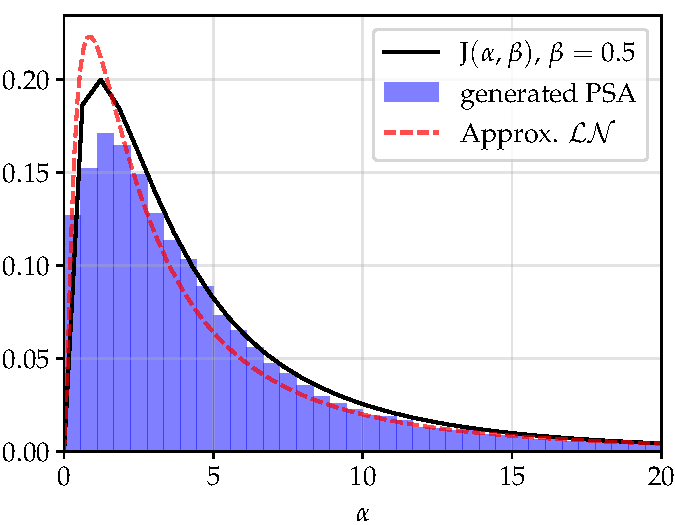
\includegraphics[width=5.2cm]{figures/PREM/PSAjeff.pdf}
        \hspace*{0.5cm}
        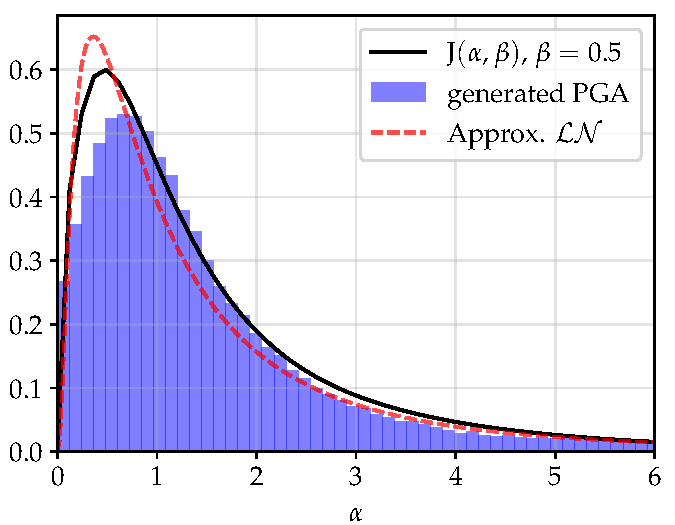
\includegraphics[width=5.2cm]{figures/PREM/PGAjeff.pdf}
        \caption{%
        Comparison of a sectional view of the Jeffreys' prior w.r.t. $\alpha$ (black) with the histograms of the generated signals (blue) and the log-normal approximations (red) for both IMs (PSA in the left figure, PGA in the right figure).
        %Comparison of a sectional view of the Jeffreys prior w.r.t. $\alpha$ (blue line) with some PGA distributions: approximated distribution of real accelerograms via Gaussian kernels in red, histogram of the generated signals in gray, and log-normal fit of the distribution in black.
        }
        \label{fig:IM}
    \end{figure}

    In practice, the use of Markov Chain Monte-Carlo (MCMC) methods (see \cref{sec:PREM:competing}) to sample the \emph{a posteriori} distribution means that the prior must be evaluated (up to a multiplicative constant) many times during the calculations. Considering the computational complexity stemming from the integrals that need to be calculated, it was decided to perform the evaluations of the prior on an experimental design based on a fine-mesh regular linear grid of $\Theta$ (here $(0,+\infty)^2$) and to build an interpolated approximation of the Jeffreys prior matching this design. This strategy is more suitable for our numerical applications and very tractable because $\Theta$ is a two-dimensional domain. \Cref{fig:jeff_prior} shows plots of the Jeffreys prior for the two IMs considered. To be precise, $2000\times2000$ prior values were computed for 
    $(\alpha,\beta)\in[10^{-5},50]\times[10^{-5},2]$ in the case of the PSA, and
    $(\alpha,\beta)\in[10^{-5},10]\times[10^{-3},2]$ in the case of the PGA. %and $\alpha\in[]$ and $\beta\in[10^{-3},2]$ and 
    These values are then processed in order to obtain a linear interpolation. 
 
    \begin{figure}[h] %[!ht]
        \centering
        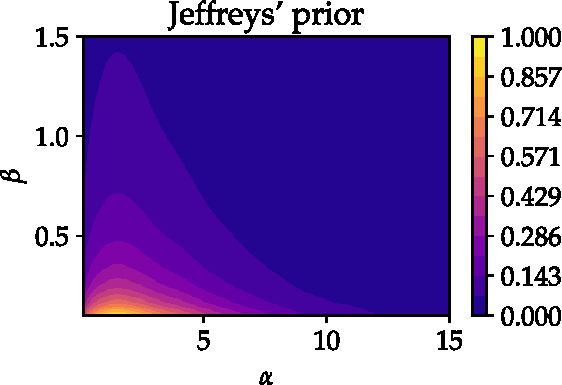
\includegraphics[height=3.8cm]{figures/PREM/Jeff_prior_PSA-1.pdf}\hspace*{0.5cm}
        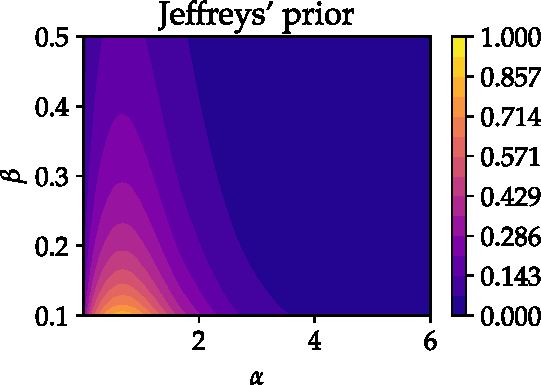
\includegraphics[height=3.8cm]{figures/PREM/Jeff_prior_PGA-2.pdf}
        %\includegraphics[width=220pt]{figures/Jeffreys_prior.pdf}%\includegraphics[height=0.4\linewidth]{figures/}
        \caption{The Jeffreys priors calculated from PSA (left) and PGA (right) on subdomains of $\Theta=(0,+\infty)^2$.}
        \label{fig:jeff_prior}
    \end{figure}
    
    %\subsection{Discussion}\label{sec:JeffDiscussion}







    The computational complexity of the Jeffreys prior is not in itself a major drawback. Since it depends exclusively on the distribution of the IM, the initial cost of the Jeffreys prior’s complex calculation would quickly be recovered in installations such as nuclear power plant, where it is necessary to determine the fragility curves of many Structures and Components (SCs). Compared to methodologies that aim to define a prior based on mechanical calculations which are, by definition, specific to SCs, the generic character of the Jeffreys prior is a clear advantage. This will be explored in the applications section of this paper (\cref{sec:PREM:numapp}). %Section~ {sec:application}). 
    Moreover, the Jeffreys prior is completely defined and does not depend on any additional subjective choices. 
    
    %The Jeffreys prior is known to be improper in numerous common cases (i.e., it cannot be normalized as a probability). This is relevant to our study, as evidenced in  {app:asymptotics}, where a calculation of the asymptotic behavior for different limits of $\theta = (\alpha,\beta)$ shows that the Jeffreys prior is indeed improper in our case. However, this characteristic is not an issue since our study focuses on the posterior, which is itself proper, as proven in  {app:asymptotics}. This is a critical issue, since MCMC algorithms would not make any sense if the posterior were improper. These asymptotic expansions also provide complementary and essential insight into the Jeffreys prior. They make it possible to understand that its behavior in $\alpha$ is similar to that of a log-normal distribution having the same median as that of the IM (i.e., here 1.1~m/s$^2$) with a variance calculated as the sum of the variance of the IM and of a term that depends on $\beta$. Figure~ {fig:IM} clearly illustrates this result.
    



    \subsection{Thorough study of the prior's decay rates}\label{sec:PREM:subsec:jeffasymp}


    Since the Jeffreys prior is known to be often improper, we propose in this section to determine its asymptotic decay rates. In   \cref{sec:PREM:degeneracy}, the decay rates of the likelihood will be computed as well, leading us to elucidate whether the posteriors yielded by Jeffreys prior are propers or not.

    We focus on the asymptotic behavior of Jeffreys in four bounds of the space $\Theta$, the study is compiled in the following propositions. 
    The statements rely on the assumption below about the distribution of the IM. %This assumption is the most appropriate 
    The comparison in \cref{fig:IM} illustrates the correctness of this assumption.


    \begin{assu}
        The IM is distributed according to a log-normal distribution, i.e., there exists $\mu\in \RR$ and $\sigma\in (0,+\infty)$ such that 
    \begin{equation}
        h(a) = \frac{1}{\sqrt{2\pi\sigma^2}a}\exp\left({-\frac{(\log a-\mu)^2}{2\sigma^2}}\right).
    \end{equation}
    \end{assu}
    %propositions that are developed below.
    %They are preceded by  the statement of two useful lemmas.

    \begin{prop}\label{prop:jeffb0}
        Fixing $\alpha>0$, there exists a $D'(\alpha)>0$ such that
            \begin{equation}
               J(\theta)\equi{\beta\rightarrow0} \frac{D'(\alpha)}{\beta}.
            \end{equation}
    \end{prop}

    \begin{prop}\label{prop:jeffbinf}
        %    Fix $\alpha>0$, there exists a constant $E'>0$ such that
        {There exists a constant $E'>0$ such that for any $\alpha>0$}
            \begin{equation}
                J(\theta)\equi{\beta\rightarrow\infty}\frac{E'}{\alpha\beta^3}.
            \end{equation}
        \end{prop}
        
        \begin{prop}\label{prop:jeffalph}
            Fixing $\beta>0$, there exists a $G''(\beta)>0$ such that
            \begin{equation}
            J(\theta) \equi{|\log\alpha|\rightarrow\infty} G''(\beta)\frac{|\log\alpha|}{\alpha}\exp\left(-\frac{(\log\alpha-\mu)^2}{2\beta^2+2\sigma^2}\right). 
        \end{equation}
        \end{prop}


    To prove these statements, we rely on the two following lemmas, which provide upper bounds for the function $\gamma\mapsto[\Phi(\gamma)(1-\Phi(\gamma))]^{-1}$.



     \begin{lem}\label{lem:phi(1-phi)ineq1}
        For any $\gamma\in\RR$, $[\Phi(\gamma)(1-\Phi(\gamma))]^{-1}\leq4\exp\left(2\gamma^2/\pi\right)$.
     \end{lem}

     \begin{lem}\label{lem:phi(1-phi)ineq2} For any $\gamma\in\RR$,
        \begin{equation}
        \Phi(\gamma) (1-\Phi(\gamma)) \geq \frac{\sqrt{2/\pi}\exp(-\gamma^2/2)}{  (|\gamma|+\sqrt{\gamma^2+4}) }. 
    \end{equation}
        
    \end{lem}


     \begin{proof}[Proof of \cref{lem:phi(1-phi)ineq1}]
        From the following inequality about the $\erf$ function \citep{chu_bounds_1955}:
\begin{equation}
        \forall \gamma>0,\, \sqrt{1-e^{-\frac{\gamma^2}{2}}}\leq\erf(\gamma/\sqrt{2})\leq\sqrt{1-e^{-2\frac{\gamma^2}{\pi}}},
    \end{equation}
we can deduce that, for any $\gamma>0$,
\begin{equation}
\begin{aligned}
    e^{-\frac{2\gamma^2}{\pi}}\hspace*{-3pt}&\leq 1-\erf(\gamma/\sqrt{2})^2\leq e^{-\frac{\gamma^2}{2}} ,  \\
    \frac{1}{4}e^{-\frac{2\gamma^2}{\pi}}\hspace*{-3pt}&\leq\frac{1}{4}\left(1-\erf\left({\gamma}/{\sqrt{2}}\right)\right)\left(1+\erf\left({\gamma}/{\sqrt{2}}\right)\right)\leq\frac{1}{4} e^{-\frac{\gamma^2}{2}}  , 
\end{aligned}
\end{equation}
the middle term being equal to $\Phi(\gamma)(1-\Phi(\gamma))$. This implies that:
\begin{equation}
    [\Phi(\gamma)(1-\Phi(\gamma))]^{-1}\leq 4 e^{\frac{2\gamma^2}{\pi}} ,
\end{equation}
hence the result for $\gamma>0$.

While it is clear that the inequality still stands for $\gamma=0$, notice that from $\Phi(-\gamma)=1-\Phi(\gamma)\,\forall\gamma\in\RR$ it follows that $\gamma\mapsto\Phi(\gamma)(1-\Phi(\gamma))$ is an even function. Thus, the inequality still stands for any $\gamma<0$; this concludes the proof of the lemma.
     \end{proof}



\begin{proof}[Proof of \cref{lem:phi(1-phi)ineq2}]
    Komatsu's inequality \citep[p.~17]{ito_diffusion_1974}:
    \begin{equation}
        \forall \gamma>0,\, \frac{2}{\sqrt{\gamma^2+4}+\gamma}\leq e^{\frac{\gamma^2}{2}}\hspace*{-4pt}\int_\gamma^\infty\hspace*{-4pt} e^{-\frac{t^2}{2}}dt\leq \frac{2}{\sqrt{\gamma^2+2}+\gamma}
    \end{equation}
    implies
    \begin{equation}
        \forall \gamma>0,\, \frac{2e^{-\frac{\gamma^2}{2}}}{\sqrt{\gamma^2+4}+\gamma}\leq\hspace*{-3.5pt} \sqrt{2\pi}(1-\Phi(\gamma)) \leq\hspace*{-2pt} \frac{2e^{-\frac{\gamma^2}{2}}}{\sqrt{\gamma^2+2}+\gamma} .
    \end{equation}
    Since $0<\Phi<1$ it follows for $\gamma>0$ that:
    \begin{equation}
        \Phi(\gamma)(1-\Phi(\gamma)) \geq \frac{2e^{-\frac{\gamma^2}{2}}}{\sqrt{\gamma^2+4}+\gamma}\left(1-\frac{2e^{-\frac{\gamma^2}{2}}}{\sqrt{\gamma^2+2}+\gamma}\right)
            \geq \frac{\sqrt{2/\pi}e^{-\frac{\gamma^2}{2}}}{\sqrt{\gamma^2+4}+\gamma}.
    \end{equation}
    Finally, since $\Phi(-\gamma)=1-\Phi(\gamma)$, $\gamma\mapsto\Phi(\gamma)(1-\Phi(\gamma))$ is an even function and we obtain for any $\gamma\in\RR$
    \begin{equation}
        \Phi(\gamma)(1-\Phi(\gamma))\geq \frac{\sqrt{2/\pi}e^{-\frac{\gamma^2}{2}}}{\sqrt{\gamma^2+4}+|\gamma|}.
    \end{equation}
\end{proof}






\subsubsection{Proofs of the propositions}
\begin{proof}[Proof of \cref{prop:jeffb0}]
    Let $\alpha>0$. For $0\leq k\leq2$, let us consider $A_{k1,k2}=A_{k1}+A_{k2}$ with $A_{kj}$ defined in \cref{eq:Aij}:
\begin{equation}
    A_{k1,k2} =  \int_{0}^{\infty}\log^k\frac{a}{\alpha}\frac{\Phi'(\gamma(a))^2}{\Phi(\gamma(a))(1-\Phi(\gamma(a)))}h(a)da .
\end{equation}
A substitution gives
    \begin{equation}
        \label{eq:AkAk}
        A_{k1,k2} =   \beta^{k+1}\int_{-\infty}^\infty  F_{A_{k1,k2}}(\gamma)d\gamma , \quad\text{with}\quad
        F_{A_{k1,k2}}(\gamma) =  \frac{\gamma^k}{2\sqrt{\pi^3\sigma^2}} \frac{e^{-\gamma^2}e^{-\frac{(\beta\gamma-\mu+\log\alpha)^2}{2\sigma^2}}}{\Phi(\gamma)(1-\Phi(\gamma))} .
    \end{equation}
%\antoine{
%Let us on another hand state the following useful inequality which we demonstrate later.
%\begin{lem}\label{lem:phiineq}
%    For any $\gamma\in\RR$, $[\Phi(\gamma)(1-\Phi(\gamma)]^{-1}\leq4\exp\left(2\gamma^2/\pi\right)$.
%\end{lem}
%}
%We remind on another hand the following inequality about the $\erf$ function (see \cite{Chu1955}):
%    \begin{equation*}
%        \forall \gamma>0,\, \sqrt{1-e^{-\gamma^2}}\leq\erf(\gamma)\leq\sqrt{1-e^{-4\frac{\gamma^2}{\pi}}}
%    \end{equation*}
%which gives using $\Phi(-\gamma)=1-\Phi(\gamma)$,
    % \begin{equation}\label{eq:Jasymp:Phiineq}
    %     \forall \gamma\in\RR,\, [\Phi(\gamma)(1-\Phi(\gamma))]^{-1}\leq4e^{2\frac{\gamma^2}{\pi}}.
    % \end{equation}
Using \cref{lem:phi(1-phi)ineq1} an upper bound can be derived for $F_{A_{k1,k2}}$: for any $\gamma\in\RR,\,\beta>0$,
\begin{equation}\label{eq:Jasymp:majFkk}
    |F_{A_{k1,k2}}(\gamma)|\leq \tilde C(\alpha)|\gamma|^ke^{-\frac{1}{3}\gamma^2},
\end{equation}
which defines an integrable function on $\RR$, $\tilde C$ being a constant independent of $\gamma$ and $\beta$. Hence the limit
\begin{equation}
    \lim_{\beta\rightarrow0}\int_{-\infty}^\infty F_{A_{k1,k2}}(\gamma)d\gamma =\hspace*{-3pt} \int_{-\infty}^\infty \frac{\gamma^k}{2\sqrt{\pi^3\sigma^2}}\frac{e^{-\gamma^2}e^{-\frac{(\mu-\log\alpha)^2}{2\sigma^2}}}{\Phi(\gamma)(1-\Phi(\gamma))}d\gamma.
\end{equation}
{%
The last integral is null when $k=1$ since the integrand is odd in this case.
When $k$ is even, the integrand is positive valued almost everywhere, which implies that the integral is positive. 
From this, we can establish that  $A_{k1,k2}\equi{\beta\rightarrow0}D_k(\alpha)\beta^{k+1}$ for some $D_k(\alpha)>0$ if $k=0,2$, and $A_{11,12}\aseq{\beta\rightarrow0}o(\beta^2)$.}

Looking back at the Fisher information matrix, we can state that
    \begin{equation}
        \det\cI(\theta)\aseq{\beta\rightarrow0}\frac{D_0(\alpha)D_2(\alpha)}{\alpha^4\beta^2} + o\left(\frac{1}{\beta^2}\right).
    \end{equation}
Finally, we obtain:
\begin{equation}\label{eq:Jrate}
    J(\theta)\equi{\beta\rightarrow0} \frac{D'(\alpha)}{\beta},
\end{equation}
where $D'(\alpha)>0$ is a constant independent of $\beta$.
\end{proof}





\begin{proof}[Proof of \cref{prop:jeffbinf}]

The asymptotic expansion of the $\erf$ function in $0$ is:
    \begin{equation}
        \erf(\gamma)\aseq{\gamma\rightarrow0}\frac{2}{\sqrt{\pi}} \gamma+O(\gamma^2) ,
    \end{equation}
which allows us to state the behavior of $\Phi(\gamma)$ when $\gamma\to0$: 
\begin{equation}
    \Phi(\gamma)\aseq{\gamma\rightarrow0} \frac{1}{2} + \frac{1}{\sqrt{2\pi}} \gamma+O(\gamma^2).    
\end{equation}
 
Let us now fix $\alpha>0$ and consider $A_{k1,k2}= A_{k1}+A_{k2}$ written as:
\begin{equation}
   A_{k1,k2} = \int_{-\infty}^\infty \tilde F_{A_{k1,k2}}(x)dx, \quad\text{with}\quad
    \tilde F_{A_{k1,k2}}(x) = \frac{x^k}{2\sqrt{\pi^3\sigma^2}}\frac{e^{-\frac{x^2}{\beta^2}}e^{-\frac{(x-\mu+\log\alpha)^2}{2\sigma^2}}}{\Phi(\beta^{-1}x)(1-\Phi(\beta^{-1}x))}.
        %&= \int_{0}^{+\infty}F_{A_{k1,k2}}(x)dx + \int_{-\infty}^0F_{A_{k1,k2}}(x)dx \nonumber\\
        %&= A_{k1,k2}^+ + A_{k1,k2}^- \label{eq:binf:splitAk}
\end{equation}
Let us note the convergence of $\tilde F_{A_{k1,k2}}(x)$ towards %$\frac{2x^k}{\sqrt{\pi^3\sigma^2}}e^{-\frac{(x-\mu+\log\alpha)^2}{2\sigma^2}}$ which defines a function in $L^1(\RR)$.
an integrable function when $\beta\to\infty$.
Moreover, \cref{lem:phi(1-phi)ineq1} allows us to bound $\tilde F_{A_{k1,k2}}$:
\begin{equation}
    |\tilde F_{A_{k1,k2}}(x)|\leq \frac{2|x|^k}{\sqrt{\pi^3\sigma^2}}e^{-\frac{(x-\mu+\log\alpha)^2}{2\sigma^2}} e^{2\frac{x^2}{\pi\beta^2}} 
        \leq \frac{2|x|^k}{\sqrt{\pi^3\sigma^2}} e^{-\frac{(x^2-2(\mu-\log\alpha))^2}{4\sigma^2}} e^{\frac{(\mu+\log\alpha)^2}{2\sigma^2}} ,
\end{equation}
for any $x\in\RR$ and $\beta>2\sigma/\sqrt{\pi}$. This dominating function is integrable on $\RR$. Thus, when $\beta\to\infty$, $A_{k1,k2}$ admits a limit expressed by:
\begin{equation}
    \lim_{\beta\rightarrow\infty}A_{k1,k2} = E_k(\alpha) = \int_{-\infty}^\infty\frac{2x^k}{\sqrt{\pi^3\sigma^2}}e^{-\frac{(x-\mu+\log\alpha)^2}{2\sigma^2}} dx= \frac{2\sqrt{2}}{\pi}\EE[X^k] ,
\end{equation}
with $X\sim\cN(\mu-\log\alpha,\sigma^2)$.
Recalling the expression of the Jeffreys prior:
    \begin{equation}
        J(\theta)^2 = \left|\frac{1}{\alpha^2\beta^6}A_{01,02}A_{21,22} - \frac{1}{\alpha^2\beta^6}A_{11,12}^2\right| ,
    \end{equation}
    we can deduce that it is equivalent to $(E_0(\alpha)E_2(\alpha)-E_1^2(\alpha))/\alpha^2\beta^6$ when $\beta\to\infty$.
    Finally,
    \begin{equation}
        J(\theta)\equi{\beta\rightarrow\infty}\frac{E'}{\alpha\beta^3} ,
    \end{equation}
with $E'=\sqrt{E_0(\alpha)E_2(\alpha)-E_1^2(\alpha)} = 2 \sigma /\pi$.

\end{proof}



\begin{proof}[Proof of \cref{prop:jeffalph}]
    
As a preliminary result, let us recall that $\erf(x)\aseq{x\rightarrow\infty}1-\frac{e^{-x^2}}{x\sqrt{\pi}} + o\left(\frac{e^{-x^2}}{x}\right)$, to establish
%use \cref{eq:Jasymp:phiasymp} to obtain
\begin{equation}\label{eq:Jasymp:Phi(1-Phi)equi}
    \Phi(\gamma)(1-\Phi(\gamma))\equi{|\gamma|\to\infty} \frac{e^{\frac{-\gamma^2}{2}}}{|\gamma|\sqrt{2\pi}}.
\end{equation}
% and we remind Komatsu's inequality:
% \begin{equation}\label{eq:komatsu}
%     \Phi(x) (1-\Phi(x)) \geq 1/ [ \sqrt{2\pi} (|x|+\sqrt{x^2+4}) ] \exp(-x^2/2)
% \end{equation}

%and to notice the monotony of $\Phi$ and its property $0<\Phi<1$, which precise the last result with the inequality
%\begin{equation}\label{eq:Jasymp:Phi(1-Phi)ineq}
%    \forall\gamma\in\RR,\, \Phi(\gamma)(1-\Phi(\gamma)) \geq \frac{e^{\frac{-\gamma^2}{2}}}{|\gamma|\sqrt{2\pi}}.
%\end{equation}

Let us consider $A_{k1,k2}=A_{k1}+A_{k2}$:
\begin{equation}
     A_{k1,k2} = C'\int_0^{\infty}\left(\log\frac{a}{\alpha}\right)^k\frac{e^{-\frac{1}{\beta^{2}}\log^2\frac{a}{\alpha}}e^{-\frac{(\log a-\mu)^2}{2\sigma^2}}}{\Phi(\beta^{-1}\log\frac{a}{\alpha})\left(1-\Phi(\beta^{-1}\log\frac{a}{\alpha})\right)}\frac{da}{a},
\end{equation}
denoting $C'=\sqrt{4\pi^3\sigma^2}^{-1}$. By substituting
\begin{equation}
    \nu = \log a - \frac{\sigma^2}{\sigma^2+ \beta^2}\log\alpha - \frac{\beta^2}{\sigma^2+\beta^2}\mu = \log a -r\log\alpha - s\mu,
\end{equation}
we obtain
\begin{equation}%\label{eq:Jasymp:Ak_nu}
     A_{k1,k2} = C'\int_{-\infty}^\infty \hat F_{A_{k1,k1}}(\nu)d\nu , 
\end{equation}
with
\begin{equation}
    \hat F_{A_{k1,k1}}(\nu)=   (\nu+(r-1)\log\alpha +s\mu)^k\frac{e^{-\frac{(\nu + (r+1)\log\alpha +s\mu)^2 }{\beta^2} } e^{-\frac{(\nu +r\log\alpha+ (s-1)\mu)^2}{2\sigma^2}}}{\left[\Phi(1-\Phi)\right](h_\beta(\nu))} ,
\end{equation}
and where $h_\beta(\nu)=\beta^{-1}(\nu+(r-1)\log\alpha+s\mu)$. Using \cref{eq:Jasymp:Phi(1-Phi)equi}, we obtain
\begin{equation}\label{eq:Jasymp:phi1phinurs}
    \left[\Phi(1-\Phi)\right](h_\beta(\nu))\hspace*{-2pt} \equi{|\log\alpha|\rightarrow\infty} \hspace*{-1pt}\frac{\beta e^{-\frac{(\nu+(r-1)\log\alpha+s\mu)^2}{2\beta^2}}}{|\nu + (r-1)\log\alpha + s\mu|\sqrt{2\pi}}.
\end{equation}
Then for a clear understanding of the asymptotic behavior of $\hat F_{A_{k1,k2}}$, let us compute 
\begin{equation}
    \begin{aligned}
        % \nonumber
     -&\frac{(\nu + (r-1)\log\alpha +s\mu)^2 }{2\beta^2} - \frac{(\nu +r\log\alpha+ (s-1)\mu)^2}{2\sigma^2} \\
% \nonumber
=& -\left(\frac{1}{2\beta^2}+\frac{1}{2\sigma^2}\right)\nu^2 -\left(\frac{((r-1)\log\alpha+s\mu)^2}{2\beta^2} +\frac{(r\log\alpha+(s-1)\mu)^2}{2\sigma^2}\right)%\nonumber
\\
         =& -\left(\frac{1}{2\beta^2}+\frac{1}{2\sigma^2}\right)\nu^2 - \frac{(\log\alpha - \mu )^2}{2(\beta^2+\sigma^2)}.
\label{eq:Jasymp:nurs}
    \end{aligned}
\end{equation}
We expand $\hat F_{k1,k2}(\nu) = \sum_{j=1}^kC_k^j(r-1)^j\log^j\alpha(\nu+s\mu)^{k-j}g(\nu)$ $ = \sum_{j=0}^k\hat F_{k1,k2}^{(j)}(\nu)$, with $g(\nu)$ defined as    \begin{equation}
        g(\nu) = \frac{e^{-\frac{(\nu + (r+1)\log\alpha +s\mu)^2 }{\beta^2} } e^{-\frac{(\nu +r\log\alpha+ (s-1)\mu)^2}{2\sigma^2}}}{\left[\Phi(1-\Phi)\right](\beta^{-1}(\nu + (r-1)\log\alpha + s\mu))}.
    \end{equation}
Therefore, by combining \cref{eq:Jasymp:phi1phinurs,eq:Jasymp:nurs}, we obtain that $\hat F_{k1,k2}^{(j)}$ satisfies
    \begin{equation}
         \hat F_{k1,k2}^{(j)}(\nu)e^{\frac{(\log\alpha-\mu)^2}{2\beta^2+2\sigma^2}}(\log\alpha)^{-j}|\log\alpha|^{-1} 
            \conv{|\log\alpha|\rightarrow\infty} (\sqrt{2\pi}\beta)^{-1}C_k^j(-1)^j(1-r)^{j+1}(\nu+s\mu)^{k-j} e^{-\left(\frac{1}{2\beta^2}+\frac{1}{2\sigma^2}\right)\nu^2}.
    \end{equation}
Using \cref{lem:phi(1-phi)ineq2}, we can also define an integrable upper bound for the above function as: %in the form of an integrable function expressed as
\begin{equation}
    |\hat F_{k1,k2}^{(j)}(\nu)|e^{\frac{(\log\alpha-\mu)^2}{2\beta^2+2\sigma^2}}|\log\alpha|^{-j-1} \leq \frac{\sqrt{2/\pi}e^{-\left(\frac{1}{2\beta^2}+\frac{1}{2\sigma^2}\right)\nu^2}}{ |h_\beta(\nu)|+\sqrt{h_\beta(\nu)^2+4}} \leq\frac{1}{\sqrt{2\pi}}e^{-\left(\frac{1}{2\beta^2}+\frac{1}{2\sigma^2}\right)\nu^2}.
\end{equation}
Thus, we can switch the limits and the integration, and the following results are obtained:
\begin{align}
    C''\beta A_{01,02}e^{\frac{(\log\alpha-\mu)^2}{2\beta^2+2\sigma^2}} &\aseq{\log\alpha\rightarrow\infty} (1-r)G\log\alpha - s\mu G  +o(1)\\
    C''\beta A_{11,12}e^{\frac{(\log\alpha-\mu)^2}{2\beta^2+2\sigma^2}}
        &\aseq{\log\alpha\rightarrow\infty} -(1-r)^2G\log^2\alpha - s^2\mu^2 G 
        + 2(1-r)s\mu G\log\alpha - G' + o(1),\\
%\end{align}
%\begin{align}
C''\beta A_{22,22}e^{\frac{(\log\alpha-\mu)^2}{2\beta^2+2\sigma^2}}
&\aseq{\log\alpha\rightarrow\infty} %\hspace*{-4pt}
(1-r)^3G\log^3\alpha - s^3\mu^3 G 
-3(1-r)^2s\mu G\log^2\alpha \\
&\hspace*{2em}-3(1-r)s^2\mu^2 G\log\alpha+3(1-r)G'\log\alpha  + o(1), \nonumber
\end{align}
%
% \begin{align*}
%     C''\beta A_{01,02}e^{\frac{(\log\alpha-\mu)^2}{2\beta^2+2\sigma^2}} \aseq{\log\alpha\rightarrow\infty}& (1-r)G\log\alpha - s\mu G  +o(1)\\
%     C''\beta A_{11,12}e^{\frac{(\log\alpha-\mu)^2}{2\beta^2+2\sigma^2}} \aseq{\log\alpha\rightarrow\infty} & -(1-r)^2G\log^2\alpha - s^2\mu^2 G + 2(1-r)s\mu G\log\alpha - G' + o(1)\\
%     C''\beta A_{22,22}e^{\frac{(\log\alpha-\mu)^2}{2\beta^2+2\sigma^2}} \aseq{\log\alpha\rightarrow\infty} & (1-r)^3G\log^3\alpha - s^3\mu^3 G -3(1-r)^2s\mu G\log^2\alpha \\
%         &+3(1-r)s^2\mu^2 G\log\alpha +3(1-r)G'\log\alpha  + o(1)
% \end{align*}
with $C''=(C'\sqrt{2\pi})^{-1}$, $G=\sigma\beta\sqrt{2\pi(\beta^2+\sigma^2)^{-1}}$ and $G'=G^2/2\pi$. 
This way
\begin{align}\nonumber
    (C'')^2\alpha^2\beta^{8} J(\theta)^2e^{2\frac{(\log\alpha-\mu)^2}{2\beta^2+2\sigma^2}}
      &  \aseq{\log\alpha\rightarrow\infty}\hspace*{-4pt}  
        3(r-1)^2s^2\mu^2G^2\log^2\alpha 
        + 3(r-1)^2s^2\mu^2G^2\log^2\alpha \\
        &\hspace*{2em} +3 (r-1)^2GG'\log^2\alpha 
        - 4(r-1)^2s^2\mu^2G^2\log^2\alpha \\
        &\hspace*{2em} - 2(r-1)^2s^2\mu^2G^2\log^2\alpha - 2(r-1)^2GG'\log^2\alpha %\\
        % &\hspace*{2em}
        + o(\log^2\alpha).\nonumber
\end{align}
Note that the above equality is still valid when $\log\alpha\to-\infty$. Finally,
\begin{equation}
    J(\theta) \equi{|\log\alpha|\rightarrow\infty} G''(\beta)\frac{|\log\alpha|}{\alpha}\exp\left(-\frac{(\log\alpha-\mu)^2}{2\beta^2+2\sigma^2}\right)  ,
\end{equation}
with 
\begin{align}
    G''(\beta) &=C''^{-1}(r-1)^2GG'\beta^{-4} 
        = \frac{2\sigma^3\beta^3 }{\sqrt{\pi}(\sigma^2+\beta^2)^{7/2}}. %\frac{\sigma^3\beta^3\sqrt{2\pi}^3}{\sqrt{\beta^2 + \sigma^2}^32\pi}\beta^{-4} .
\end{align}


\end{proof}

This study states that the Jeffreys prior is improper, since it is not integrable w.r.t. $\beta$.


\section{Competing approaches and estimation tools}\label{sec:PREM:competing}



    \subsection{Bayesian estimates of the seismic fragility curve}


    The most relevant method in order to benefit from the Bayesian theory and the reference prior construction presented in \cref{sec:PREM:model} consists in deriving the posterior defined in \cref{eq:PREM:posterior}.
    When the latter is proper, it then becomes possible to generate, according to that distribution, samples of $\theta$ conditioned on the observed data. These \emph{a posteriori} generations of $\theta$ can be obtained using MCMC methods. In this study, we have implemented an adaptive Metropolis-Hastings (M-H) algorithm with a Gaussian transition kernel and a covariance adaptation process (following the suggestions of \cite{haario_adaptive_2001}). Such an algorithm allows sampling from a probability density known up to a multiplicative constant. In this context, the \emph{a posteriori} samples of $\theta$ can be used to define credibility intervals for the probit-lognormal estimations of the fragility curves.



    \subsection{Competing prior taken from the literature}

    {For comparison purposes, we selected the prior} suggested by \citet{straub_improved_2008} ---called the SK prior--- whose density is defined as the product of a normal distribution for $\ln(\alpha)$ and the improper distribution $1/\beta$ for $\beta$, namely:
    \begin{equation}\label{eq:Straubprior}
        \pi_{SK}(\theta)\propto\frac{1}{\alpha\beta} \exp\Big( -\frac{(\log\alpha-\mu)^2}{2\sigma^2}\Big).
    \end{equation}
In \cite{straub_improved_2008}, the parameters $\mu$ and $\sigma$ of the log-normal distribution are chosen to generate a non-informative prior. 
%As specified in the introduction to Section~ {sec:tools}, 
For a fair comparison with the approach proposed in this chapter, we decided to pick $\mu$ and $\sigma$ as equal to the mean and the standard deviation of the logarithm of the IM. This choice is consistent with the fact that the Jeffreys prior is similar to a log-normal distribution with these parameters (see \cref{fig:IM}). The prior $\pi_{SK}(\theta)$ is plotted in \cref{fig:Straubprior} for both the PSA and the PGA as IM.

\begin{figure}[h]
    \centering
    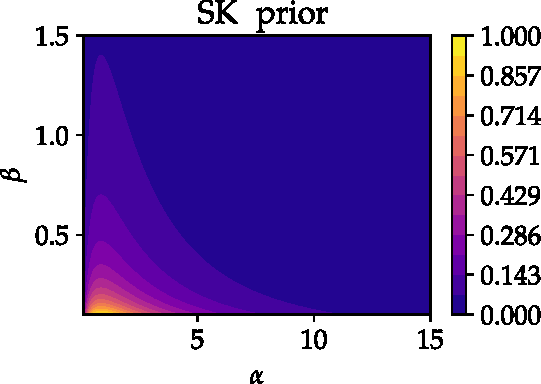
\includegraphics[width=5cm]{figures/PREM/SK_prior_PSA.pdf}\hspace*{0.5cm}
    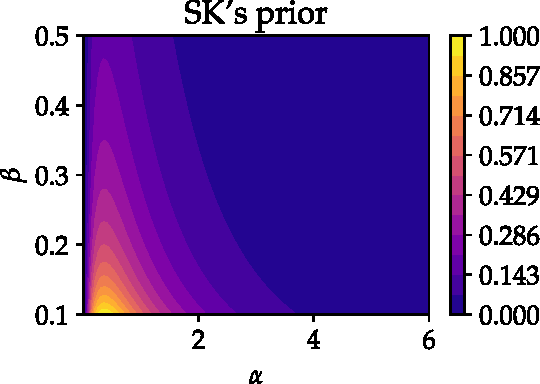
\includegraphics[width=5cm]{figures/PREM/SK_prior_PGA.pdf}
    %\includegraphics[width=210pt]{figures/SK.pdf} %height=0.4\linewidth
    \caption{Prior suggested by \citet{straub_improved_2008},  expressed in \cref{eq:Straubprior} and scaled to a log-normal estimation of the IM distribution, for both the PSA (left) and the PGA (right) as IM.}
    \label{fig:Straubprior}
\end{figure}


An analysis of the posterior obtained from the SK prior is given in \cref{sec:PREM:degeneracy}. It shows that the posterior is always improper, which jeopardizes the validity of any \emph{a posteriori} estimation using MCMC methods. This could however be mitigated by truncating w.r.t. $\beta$ (yet this involves a subjective choice), which we will do in the numerical application conducted in this work. This issue persists in the authors' original framework, which is slightly different from ours. This is confirmed in \cref{app:SKreview}.


\paragraph{Asymptotic comparison of the Jeffreys and SK priors} 
By comparing the Jeffreys and SK prior asymptotics, it can be observed that:
    \begin{itemize}
        \item Regarding the asymptotics w.r.t. $\beta$, while the divergence rates are the same when $\beta\to0$, the Jeffreys prior performs better when $\beta\to\infty$:
            \begin{equation}
                J(\theta) \underset{\beta\rightarrow\infty}{\propto} \beta^{-2}\pi_{SK}(\theta).
            \end{equation}
        Consequently, the SK posterior will result in higher probabilities for high values of $\beta$ compared to the Jeffreys prior.
        \item Regarding the asymptotics w.r.t. $\alpha$, both are asymptotically close to a log-normal distribution, with a slight ``disadvantage'' for the Jeffreys prior, for which the asymptotic variance is derived by adding $\beta^2$ to the variance of the SK prior. This means that while for small values of $\beta$ (smaller than $\sigma$), both priors remain comparable w.r.t. $\alpha$, the Jeffreys prior gives higher probabilities to $\alpha$ outliers when $\beta$ also has a high value. However, as seen above, the probability for large values of $\beta$ is quite low for the Jeffreys prior compared to the SK prior. %This explains why the generation of such $\alpha$ outliers has not been observed in the estimations presented in this paper.
    \end{itemize}


% \paragraph{}
%


    \subsection{Maximum likelihood estimation with bootstrapping}

The most common non-Bayesian estimator of the seismic fragility curves under the probit-lognormal modeling is the maximum likelihood estimator (MLE). This estimator has been introduced in   \cref{chap:frags-intro} (\cref{sec:intro-frags:models}). It is expressed as follows given a set of $k$ observations $(\mbf z^k,\mbf a^k)$:
    \begin{equation}
        \theta^{\text{MLE}}(\mbf z^k,\mbf a^k)=\argmax_{\theta\in\Theta}\ell_k(\mbf z^k|\mbf a^k,\theta).
    \end{equation}
    %$\theta^{\text{MLE}}(\mbf z^k,\mbf a^k)=\argmax_{\theta\in\Theta}\ell_k(\mbf z^k,\mbf a^k|\theta)$.
It is common to compute multiple MLE in order to obtain confidence intervals. Doing so, the bootstrap technique defines the stochastic estimator of $\theta$:
    \begin{equation}
        \hat\theta_k^{\text{BMLE}}(\mbf z^k,\mbf a^k) = \theta^{\text{MLE}}((z_{U_i},a_{U_i})_{i=1}^k),
    \end{equation}    
  where $U_1,\dots,U_k$ are i.i.d. random variables distributed w.r.t. a uniform distribution in $\{1,\dots,k\}$.
This estimator is used to compute confidence intervals by estimating empirically its quantiles from many samples. 
This is a very common approach for fragility curves (e.g., 
\cite{shinozuka_statistical_2000,gehl_influence_2015,baker_efficient_2015}). The convergence of the MLE and the relevance of this method are detailed in \cite{van_der_vaart_asymptotic_1992}. However, the relevance of the bootstrap method is often limited by the irregularity of its results for small values of $k$ (see e.g., \cite{zentner_fragility_2017}).





\section{Limits of the estimates given by the three approaches: the curse of degeneracy}\label{sec:PREM:degeneracy}

In this section, we study the likelihood decay rates in order to (i) explain irregular phenomena commonly encountered with classical frequentist methods, and (ii) verify the proper characteristics of the posteriors in the Bayesian framework.
Our study of the likelihood's asymptotic behavior is summarized in the following proposition.

\begin{prop}\label{prop:likelihood}
    Let us consider $k>1$ and a data sample $(\mbf a^k, \mbf z^k)$. 
    Let us introduce the vectors $\mbf N=(z_i\indic_{a_i<\alpha}+(1-z_i)\indic_{a_i>\alpha})_{i=1}^k$, $\log^2\frac{\mbf a^k}{\alpha}=(\log^2\frac{a_i}{\alpha})_{i=1}^k$.  
    
    \begin{itemize}
        \item Fixing $\alpha>0$, then 
        \begin{equation}
        \ell_k(\mbf z^k|\mbf a^k,\theta) \conv{\beta\rightarrow\infty}2^{-k}\quad\text{and}\quad
        % \end{equation}
% and
        % \begin{equation}
            \ell_k(\mbf z^k|\mbf a^k,\theta) \aseq{\beta\rightarrow0}O\left(\beta^{|\mbf N|}e^{-\frac{\mbf N^T\log^2\frac{\mbf a^k}{\alpha}}{2\beta^2}}\right) ,
        \end{equation}
        where $|\mbf N|=\sum_{i=1}^kN_i$.
        \item Fixing $\beta>0$, then
        \begin{equation}
            \ell_k(\mbf z^k|\mbf a^k,\theta) \hspace*{-3pt} \aseq{\alpha\rightarrow0}\hspace*{-3pt} O\left(|\log\alpha|^{|\mbf z^k|-k} e^{-\frac{1}{2\beta^2}\sum_{i=1}^k (1-z_i)(\log a_i-\log\alpha)^2} \right)
        \end{equation}
        and 
        \begin{equation}
            \ell_k(\mbf z^k|\mbf a^k,\theta) \hspace*{-3pt}\aseq{\alpha\rightarrow\infty}\hspace*{-3pt} O\left(\log(\alpha)^{-|\mbf z^k|} e^{-\frac{1}{2\beta^2}\sum_{i=1}^k z_i(\log a_i-\log\alpha)^2} \right) ,
        \end{equation}
        where $|\mbf z^k|=\sum_{i=1}^kz_i$ is the number of failures in the observed sample.
    \end{itemize}
\end{prop}



\begin{proof}[Proof of \cref{prop:likelihood}]
    As a reminder, the likelihood is expressed as:
    \begin{equation}
    \begin{aligned}%\label{eq:likelitocalc}
        \ell_k(\mbf z^k|\mbf a^k,\theta)  &= \prod_{i=1}^k\Phi\left(\frac{\log a_i-\log\alpha}{\beta}\right)^{z_i}\left(1-\Phi\left(\frac{\log a_i-\log\alpha}{\beta}\right)\right)^{1-z_i} \\
%            & = \prod_{i=1}^k\Phi(\gamma_i)^{z_i}(1-\Phi(\gamma_i))^{1-z_i}\\
            & = \exp\left[\sum_{i=1}^k\left(z_i\log\Phi(\gamma_i) + (1-z_i)\log(1-\Phi(\gamma_i))\right)\right] ,
    \end{aligned}
\end{equation}
denoting $\gamma_i=\beta^{-1}\log\frac{a_i}{\alpha}$. %\antoine{We want to study the bahavior of this expression when the $\gamma_i\to\infty$.} %, note that $\gamma\conv{\beta\rightarrow0}\eps_i\infty$ a.s. where $\eps_i=1$ if $a_i>\alpha$;  \antoine{$-1$ if $a_i<\alpha$; and $0$ otherwise.}

To treat the case where $\beta\to\infty$ we can observe that while $\alpha$ is fixed, the quantities $\Phi(\gamma_i)$ all converge to ${1}/{2}$. The product of those limits gives the limit $\ell_k(\mbf z^k|\mbf a^k,\theta)\conv{\beta\rightarrow\infty}2^{-k}$.


For the other cases, it should be reminded that $\Phi(x)=\frac{1}{2}(1+\erf(x/\sqrt{2}))$ and $\erf(x)\aseq{x\rightarrow\infty}1-\frac{e^{-x^2}}{x\sqrt{\pi}} + o\left(\frac{e^{-x^2}}{x}\right)$, which leads to 
    \begin{equation}\label{eq:Jasymp:phiasymp}
        \Phi(x)\aseq{x\rightarrow\infty}1 - \frac{e^{-\frac{x^2}{2}}}{x\sqrt{2\pi}} + o\left(\frac{e^{-\frac{x^2}{2}}}{x}\right).
    \end{equation}
Let us consider an $i\in\{1,\dots,k\}$ and compute
\begin{equation}
    \begin{aligned}
        &z_i\log\Phi(\gamma_i) + (1-z_i)\log(1-\Phi(\gamma_i)) \\
           &\qquad  \aseq{\gamma_i\rightarrow\infty} z_i\log\left(1-\frac{e^{-\frac{\gamma_i^2}{2}}}{\gamma_i\sqrt{2\pi}} + o\left(\frac{e^{-\frac{\gamma_i^2}{2}}}{\gamma_i}\right)\right)
        %   &\hspace*{2em}
          +(1-z_i)\log\left(\frac{e^{-\frac{\gamma_i^2}{2}}}{\gamma_i\sqrt{2\pi}} + o\left(\frac{e^{-\frac{\gamma_i^2}{2}}}{\gamma_i}\right)\right)\\
           &\qquad \aseq{\gamma_i\rightarrow\infty} -z_i\frac{e^{-\frac{\gamma_i^2}{2}}}{\gamma_i\sqrt{2\pi}}  %o\left(\frac{e^{-\gamma_i^2}}{\gamma_i}\right) 
                +(1-z_i)\log\left(\frac{e^{-\frac{\gamma_i^2}{2}}}{\gamma_i\sqrt{2\pi}}\right) + o(1)\\
           &\qquad \aseq{\gamma_i\rightarrow\infty} - (1-z_i)\frac{\gamma_i^2}{2} - (1-z_i)\log(\gamma_i\sqrt{2\pi}) + o(1).
    \end{aligned}
\end{equation}
Using the relation $\Phi(-x)=1-\Phi(x)$, it follows that, in the case $a_i<\alpha$:
    \begin{equation}
        z_i\log\Phi(\gamma_i) + (1-z_i)\log(1-\Phi(\gamma_i))
            \aseq{\gamma_i\rightarrow-\infty} - z_i\frac{\gamma_i^2}{2} - z_i\log(-\gamma_i\sqrt{2\pi}) + o(1).
    \end{equation}

{
Going back to the likelihood asymptotics, let us first suppose $\alpha>0$ and $\beta\to0$. Thus, denoting the vectors $\mbf N=(z_i\indic_{a_i<\alpha}+(1-z_i)\indic_{a_i>\alpha})_{i=1}^k$ and 
$\log^2\frac{\mbf a^k}{\alpha}=(\log^2\frac{a_i}{\alpha})_{i=1}^k$, we obtain
    \begin{equation}
        \ell_k(\mbf z^k|\mbf a^,\theta) \aseq{\beta\rightarrow0} \frac{C(\alpha)}{\sqrt{2\pi}^{|\mbf N|}}\beta^{|\mbf N|} e^{-\frac{\mbf N^T\log^2\frac{\mbf a^k}{\alpha}}{2\beta^2}+o(1)} %\mbox{ is a constant}
            \aseq{\beta\rightarrow0}O\left(\beta^{|\mbf N|}e^{-\frac{\mbf N^T\log^2\frac{\mbf a^k}{\alpha}}{2\beta^2}}\right) ,
    \end{equation}
where $|\mbf N|=\sum_{i=1}^kN_i$ and $C(\alpha) =\prod_{i=1}^k\left|\log\frac{a_i}{\alpha}\right|^{N_i}$. %Note that $N$

Let us then fix $\beta>0$ to get
\begin{equation}
    \begin{aligned}
        \ell_k(\mbf z^k|\mbf a^k,\theta) &\aseq{\alpha\rightarrow\infty} \frac{\beta^{|\mbf N|}}{\sqrt{2\pi}^{|\mbf N|}} \left(\prod_{i=1}^k\log\left(\frac\alpha{a_i}\right)^{-z_i}\right) 
        % &\hspace*{1.5em}\cdot 
        \exp\left({-\frac{1}{2\beta^2}\sum_{i=1}^k z_i(\log a_i-\log\alpha)^2+o(1)}\right)
        \\
            &\aseq{\alpha\rightarrow\infty}O\left(\log(\alpha)^{-|\mbf z^k|} e^{-\frac{1}{2\beta^2}\sum_{i=1}^k z_i(\log a_i-\log\alpha)^2} \right),
    \end{aligned}
\end{equation}
where $|\mbf z^k|=\sum_{i=1}^kz_i$ is the number of failures in the observed sample.
Similarly, we obtain
\begin{equation}
    \begin{aligned}
        \ell_k(\mbf z^k|\mbf a^k,\theta) 
        &\aseq{\alpha\rightarrow0}
            \frac{\beta^{|\mbf N|}}{\sqrt{2\pi}^{|\mbf N|}} \left(\prod_{i=1}^k\log\left(\frac{a_i}\alpha\right)^{-(1-z_i)}\right) 
            % &\hspace*{1.5em}\cdot 
            \exp\left({-\frac{1}{2\beta^2}\sum_{i=1}^k (1-z_i)(\log a_i-\log\alpha)^2+o(1)}\right)
        \\
            &\aseq{\alpha\rightarrow0}O\left(|\log\alpha|^{|\mbf z^k|-k} e^{-\frac{1}{2\beta^2}\sum_{i=1}^k (1-z_i)(\log a_i-\log\alpha)^2} \right).
    \end{aligned}
\end{equation}
}
\end{proof}


This statement expresses that, under general circumstances, the likelihood converges rapidly to $0$ in every direction but the one where $\beta\to\infty$.
The latter is a concern, because it requires that the decay rate of the prior in that direction is proper to yield proper posteriors.
Moreover, under some circumstances, %several problemtaic pheno
the vector $\mbf N$ is null. It is the case when we fall in one the three scenarios described in the following definition.
In that case, we say that the likelihood is degenerate, and it does not converge towards $0$ when $\beta\to0$. 


\begin{defi}[Likelihood degeneracy]\label{def:degeneracy}
    %If the observed data $(\mbf z^k,\mbf a^k)$ are such that, either,
    If the observed samples $(\mbf z^k,\mbf a^k)$ belong to one of the following three types:
    \begin{itemize}
        \item {type 1 : no failure is observed: $z_i=0$ for any $i$;}
        \item {type 2 : only failures are observed: $z_i=1$ for any $i$;}
        \item {type 3 : the failures and non-failures are partitioned into two disjoint subsets when classified according to their IM values:}
        %the failures and successes are discriminated according to their IM: 
        there exists $a\in\cA$ such that for any $i,j$, $a_i<a<a_j\Longleftrightarrow z_i\ne z_j$ (see the illustration in \cref{fig:degenerate-frag});
    \end{itemize}
    then the likelihood is degenerate.
\end{defi}



An example of degenerate likelihood is presented in \cref{fig:degenerate-frag} with an illustration of this phenomenon.
In the following, we deduce from this study the decay rates of the posterior densities 
yielded by the two priors considered in this work (the SK prior and the Jeffreys prior).
In particular, we show that the Jeffreys prior may produce improper posteriors in degenerate scenarios.
For this reason, this chapter addresses the estimation of seismic fragility curves from dataset issuing non-degenerate likelihoods.


\begin{figure}[h]
    \centering
    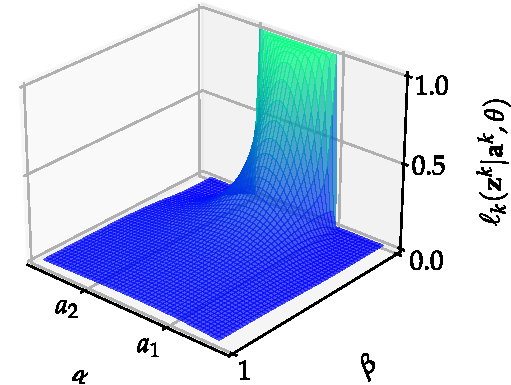
\includegraphics[width=4.6cm]{figures/PREM/likelihood_degen.pdf}\qquad
    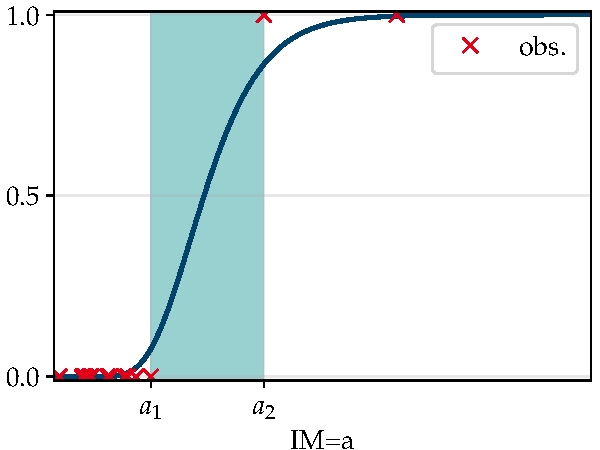
\includegraphics[width=4.44cm]{figures/PREM/degeneracy.pdf}
    \caption{{Example of a type 3 data sample $(\mbf z^k,\mbf a^k)$ which gives a degenerate likelihood. Graphs of (left) the likelihood given the degenerate data sample as a function of the tuple $(\alpha,\beta)$ and (right) the fragility curve (blue curve) according to which the points (red crosses) are sampled : each red cross is a tuple $(z,a)$, where its X-axis equals $a$ and its Y-axis equals $z$.}
    In both figures, $a_1$ is the maximal observed IM value among ``non-failures'', and $a_2$ is minimal one among ``failures''.
    The interval $(a_1,a_2)$ (in cyan in the right figure) separates the failures and the non-failure observed.
    }
    \label{fig:degenerate-frag}
\end{figure}



%limits the study to case studies where 

\subsubsection{Decay rates of the posterior densities and properness}


The Jeffreys and SK priors are not proper with respect to $\beta$ (see \cref{sec:PREM:Jeffreys} for the Jeffreys prior and \cref{eq:Straubprior} for the SK prior). For the Jeffreys prior, the divergence and convergence rates with respect to $\beta$ only make the resulting posterior proper when the prior is coupled with non-degenerate likelihoods. 
%The particular circumstances leading to a likelihood divergence when $\beta\rightarrow0$, as mentioned in  {app:lieklihood-asympt}, do not apply.
 However, one can see that this is not the case for the SK posterior, which is not integrable w.r.t. $\beta$ because of a convergence rate that is too low at $+\infty$. This prevents the validation of the MCMC estimates for this posterior, unless a truncation of the distribution is considered. %This explains the generation of \emph{a posteriori} outliers using the SK prior. 
 Note that this prior was originally designed within
%   considered this prior within 
a Bayesian framework that slightly differs from ours. In \cref{app:SKreview}, we confirm that the posterior is not proper even when derived in the exact framework of the author's paper. % \cite{Straub2008}.



% \subsection{Improperness of the SK posterior in the original framework of the authors}



% We stated above that, within our framework, the SK prior always results in an improper posterior. This puts the validity of the MCMC estimations into question, unless if the domain is truncated in $\beta$. %and could explain the lower performance of the SK prior compared to the Jeffreys prior. 
% In \cite{straub_improved_2008}, the authors use the Bayesian methodology the same way we do, yet the consideration of uncertainties over the observed earthquake intensity measures and the equipment capacities leads to a slightly different likelihood.
% In order to verify that the drawbacks of their prior highlighted in this paper are not due to our statistical choices, we dedicated this appendix to the study of the asymptotic expansions of the posterior in the exact framework presented in \cite{Straub2008}.
% We shall first introduce the exact model of \citeauthor{Straub2008} for the estimation of seismic fragility curves in  {subapp:C1}, using notations consistent with our study. We will then derive the likelihood and its asymptotics in  {subapp:C2}. Finally, we will express the convergence rates of the posterior in  {subapp:C3}, which will allow us to conclude that the SK posterior is indeed improper.





\section{Performance evaluation metrics}\label{sec:PREM:metrics}

In order to assess and compare the performances of the proposed approaches, we propose different quantitative metrics.
Beforehand, we suppose we have access to a reference fragility curve $P^{\text{ref}}_f$. In two of the case studies that we treat in the following, a large validation dataset is available and can be used to derive such reference using non-parametric Monte-Carlo estimates following the suggestion of \citet{trevlopoulos_parametric_2019}. This method was described in   \cref{chap:frags-intro} (\cref{sec:intro-frags:models}) and implemented in   \cref{chap:frags-intro} onto two case studies for which a large validation dataset was available.
%We recall briefly the construction of this reference from the validation dataset denoted $(z_i,a_i)_{i=1}^{}$.
% It follows the suggestion of \citet{trevlopoulos_parametric_2019}

Given observations $(\mbf z^k,\mbf a^k)$, we denote by $a\mapsto P_f^{|\mbf z^k,\mbf a^k}(a)$ the random process defined as the fragility curve conditional to the $(\mbf z^k,\mbf a^k)$. Its distribution inherits from the posterior distribution of $\theta$ in the case of the Bayesian method, or it inherits from the distribution of the bootstrap estimator $\hat\theta^{\text{BMLE}}(\mbf z^k,\mbf a^k)$ in the case of the MLE.
For each value $a$, the $r$-quantile of the random variable $P_f^{|\mbf z^k,\mbf a^k}(a)$ is denoted by $q_r^{|\mbf z^k,\mbf a^k}(a)$. We then define:
\begin{itemize}
    \item The quadratic error: $\cE^{|\mbf z^k,\mbf a^k}=\EE_{\theta|\mbf z^k,\mbf a^k}\left[\|P_f^{|\mbf z^k,\mbf a^k}-P_f^{\mathrm{ref}} \|^2_{L^2}\right].$
        \item The $1-r$ square credibility width: $\cW^{|\mbf z^k,\mbf a^k}= \|q_{1-{r/2}}^{|\mbf z^k,\mbf a^k} - q_{{r/2}}^{|\mbf z^k,\mbf a^k}\|_{L^2}^2$.
\end{itemize}
The $L^2$ norm is taken on the domain $[a_{\text{min}},a_{\text{max}}]$ that covers  the available seismic signals: 
\begin{equation}
    \|P\|^2_{L^2} = \int_{a_{\text{min}}}^{a_{\text{max}}} P(a)^2da.    
\end{equation}
The $L^2$ norms are approximated using Simpson's interpolation, and the expectation are estimated by Monte-Carlo sums, using samples following either the posterior distributions or the distribution of the bootstrap estimator. 









\section{Numerical applications}\label{sec:PREM:numapp}


In this section, we will examine three case studies.
Two of them leverage the many simulation datasets available that have been previously computed for validation purposes. They will be used in the derivation of a reference fragility curve (as explained in \cref{sec:PREM:metrics}), and allow us to validate the corresponding probit-lognormal models. 
The three case studies were presented in   \cref{chap:frags-intro}. The first one is a nonlinear oscillator
for which $10^5$ nonlinear simulations have been implemented for validation purposes. The second case study deals with a piping system which is part of the secondary cooling system of a French Pressurized Water Reactor. Due to the high computational cost, only $10^4$ simulations have been performed for this case. In both cases, estimations are performed using different testing data sets of a size $k$ chosen as negligible compared to the size of the validation dataset. These testing datasets are taken from the set of available nonlinear dynamical simulation results. {A third case study is eventually presented %as supplementary material 
in order to showcase how our method could be applied to practical experiments.}




\subsection{Case study 1: the elasto-plastic oscillator}

% \textcolor{orange}{description}

The first case study is a single-degree-of-freedom elasto-plastic oscillator
with kinematic hardening. This mechanical system was presented in   \cref{chap:frags-intro} (\cref{sec:intro-frags:elastoplastic}).
For this case study, $10^5$ nonlinear dynamical simulations have been conducted to constitute a validation dataset.
In \cref{fig:PREM:oscill}, we recall (i) a scheme of the oscillator, (ii) the validation dataset in the plan (PGA,EDP), (iii) reference fragility curves derived using non-parametric estimation from the validation dataset (see \cref{sec:PREM:metrics}).
In this study, the failure is defined when the EDP exceeds a threshold $C=0.8$~cm.

\begin{figure}[h]
    \centering
    \parbox[b][3.8cm][t]{5.2cm}{
        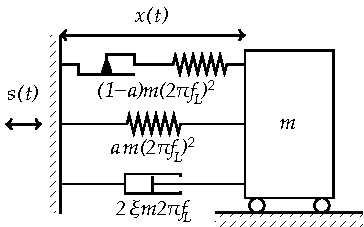
\includegraphics[height=3.2cm]{figures/intro-frags/KBEPO_rheo.pdf}}\ \ 
    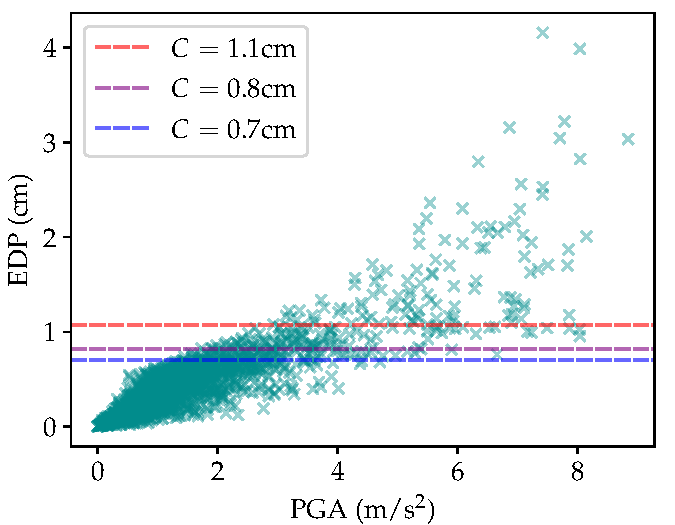
\includegraphics[height=3.8cm]{figures/intro-frags/oscill/cloudPGA.pdf}\ \ 
    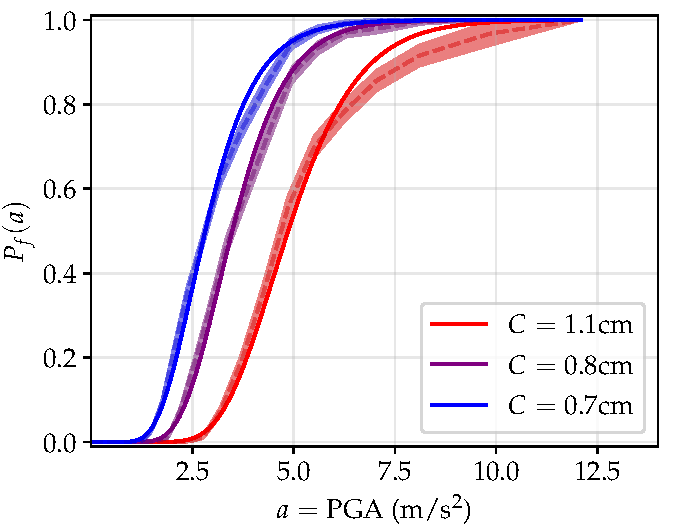
\includegraphics[height=3.8cm]{figures/intro-frags/oscill/refs_PGA.pdf}
    \caption{Illustration of the first case study. Left: scheme of an elasto-plastic oscillator of mass $m$. Middle: results of $10^5$ non-linear dynamical simulations. Right: reference non-parametric fragility curves (dashed lines) surrounded by their $95\%$-confidence intervals, compared with the probit-lognormal fragility curves derived by MLE from the validation dataset of size $10^5$. Different thresholds $C$ are considered, each yields different proportions of failures in the validation dataset: resp. $95\%$ (red), $90\%$ (purple) and $85\%$ (blue).}
    \label{fig:PREM:oscill}
\end{figure}



Examples of fragility curve estimations are shown in \cref{fig:curvesONL}. They are obtained from $5000$ samples of $\theta$ generated with the implemented statistical methods (see \cref{sec:PREM:competing}), which are based on two observation sets of sizes $k=20$ and $k=30$. Although the nature of the two intervals compared is different ---credibility interval for the Bayesian framework and confidence interval for the MLE---, these results clearly illustrate the advantage of the Bayesian framework over the MLE for small samples. With the MLE, irregularities characterized by null estimates of $\beta$ appear, resulting in ``vertical'' confidence intervals. In \cref{sec:PREM:degeneracy}, we established that the likelihood is easily maximized for $\beta=0$ when samples are partitioned into two disjunct subsets when classified according to IM values: one subset for which there is no failure and one for which there is failure (i.e. when the likelihood is degenerate because of a type 3 data sample). Moreover, when few failures are observed in the initial sample, the bootstrap technique can lead to the consideration of many sub-samples that maximize the likelihood at $\beta=0$. This is better evidenced by an examination of the raw values of $\theta$ generated in \cref{fig:scatterONL}. The degenerate $\beta$ values resulting from the MLE appear clearly but, although it should theoretically also be affected, the Bayesian framework shows no evidence of a similar phenomenon for this type of samples.


\begin{figure}[h]
    \centering%
    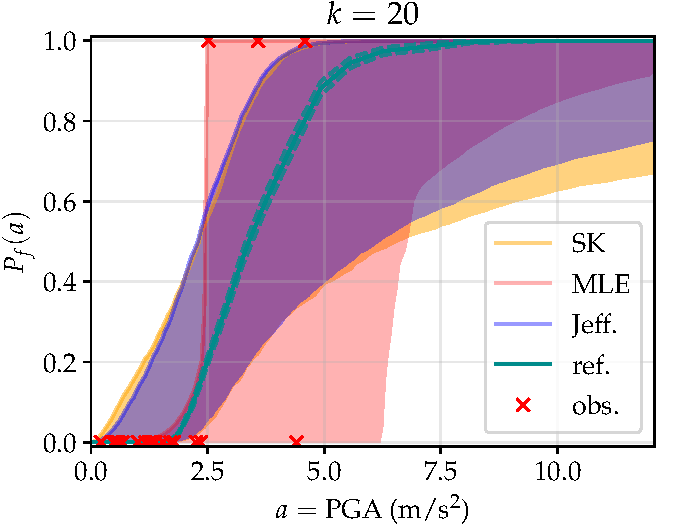
\includegraphics[width=5.2cm]{figures/PREM/oscill/PGA20.pdf}\hspace*{0.5cm}
    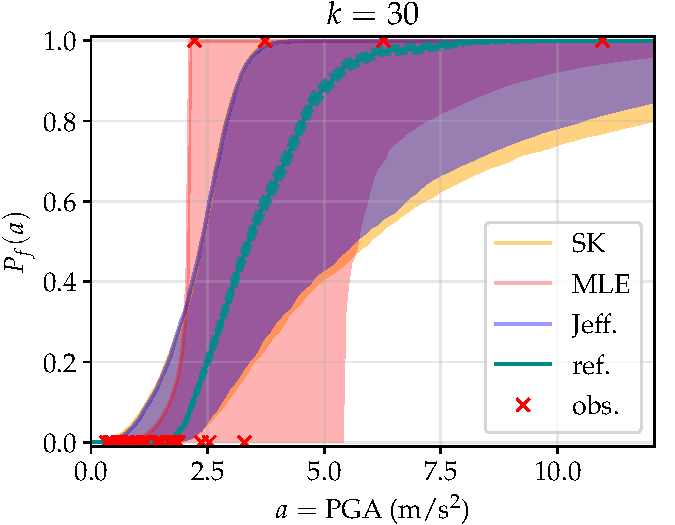
\includegraphics[width=5.2cm]{figures/PREM/oscill/PGA30.pdf}
    %\hspace*{-0.1\linewidth}\includegraphics[width=1.2\linewidth]{figures/curves.pdf}
    % 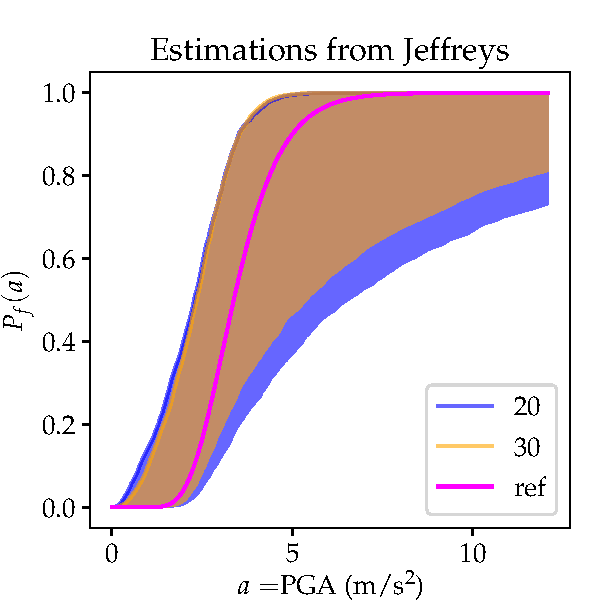
\includegraphics[width=130pt]{figures/Jeff_curves.pdf}% %0.33\linewidth
    % 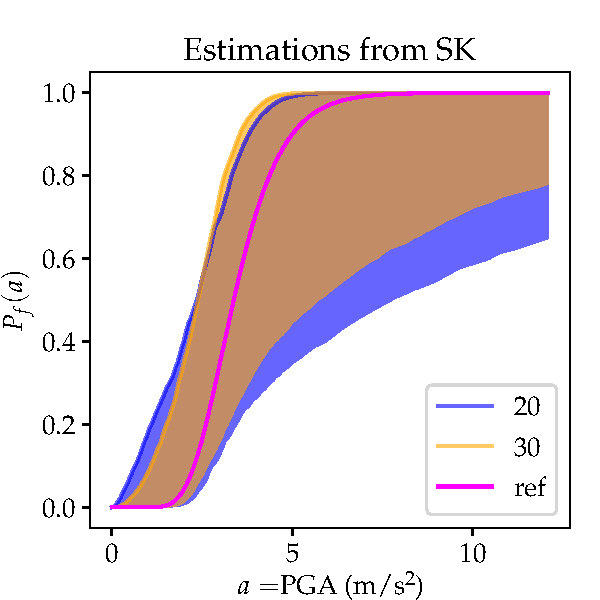
\includegraphics[width=130pt]{figures/SK_curves.pdf}%
    % 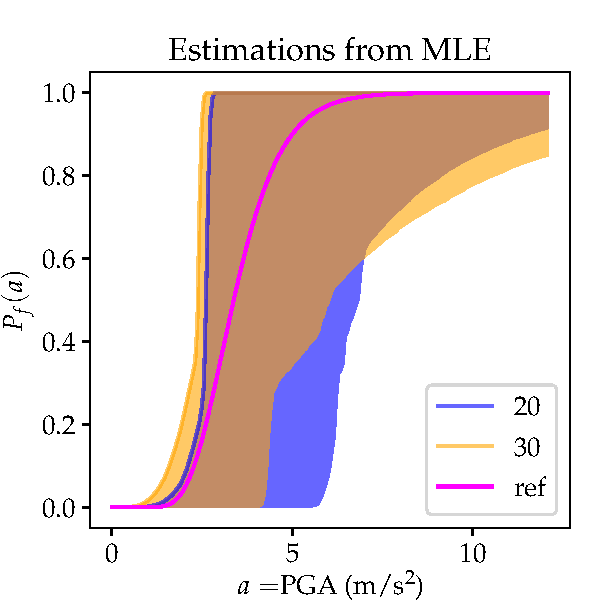
\includegraphics[width=130pt]{figures/MLE_curves.pdf}%
    \caption{$95\%$ credibility (for Bayesian estimation) or confidence (for the MLE) intervals of fragility curve estimations for the elasto-plastic oscillator, using the methods described in \cref{sec:PREM:competing}. %, obtained from a total of $5000$ estimations of $\theta$ using the {statistical methods introduced in \cref{sec:PREM:metrics}. In the left (resp. right) figure $k=20$ (resp. $k=30$) data are observed. 
    The cyan curve is the reference $P^\text{ref}_f$ suggested in \cref{sec:PREM:metrics}, surrounded by its $95\%$-confidence interval (dashed lines). The red crosses represent the observed data.}
    \label{fig:curvesONL}
\end{figure}


\begin{figure}[h]
    \centering%
    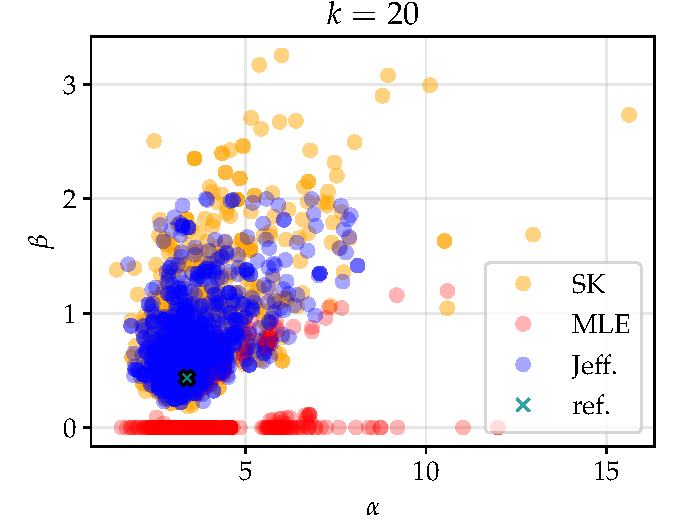
\includegraphics[width=5.2cm]{figures/PREM/oscill/PGA20scatter.pdf}\hspace*{0.5cm}
    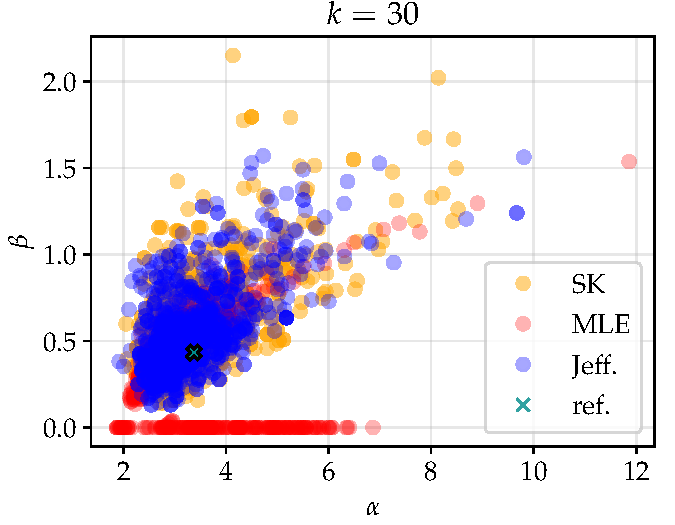
\includegraphics[width=5.2cm]{figures/PREM/oscill/PGA30scatter.pdf}
    % 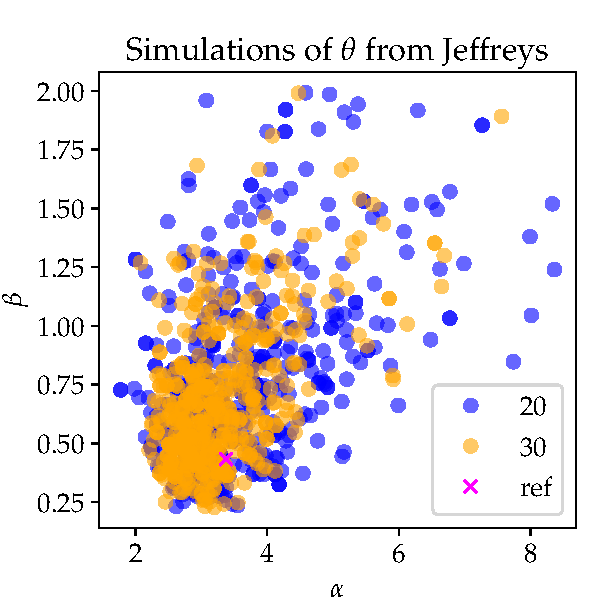
\includegraphics[width=130pt]{figures/Jeff_scat_light.pdf}%0.33\linewidth
    % 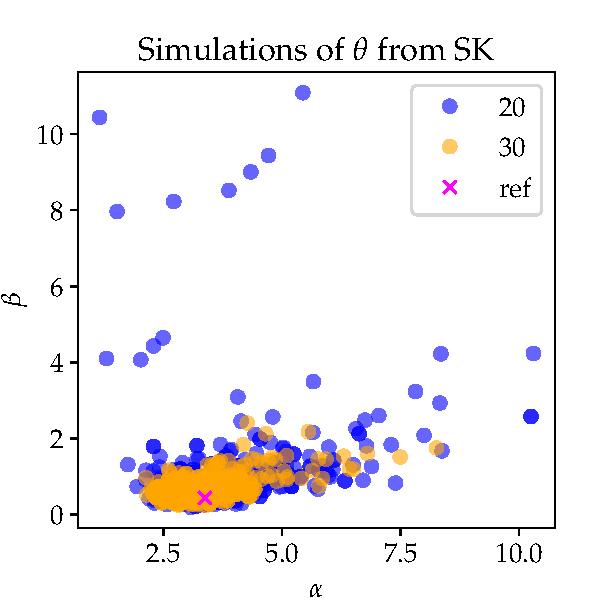
\includegraphics[width=130pt]{figures/SK_scat_light.pdf}%
    % 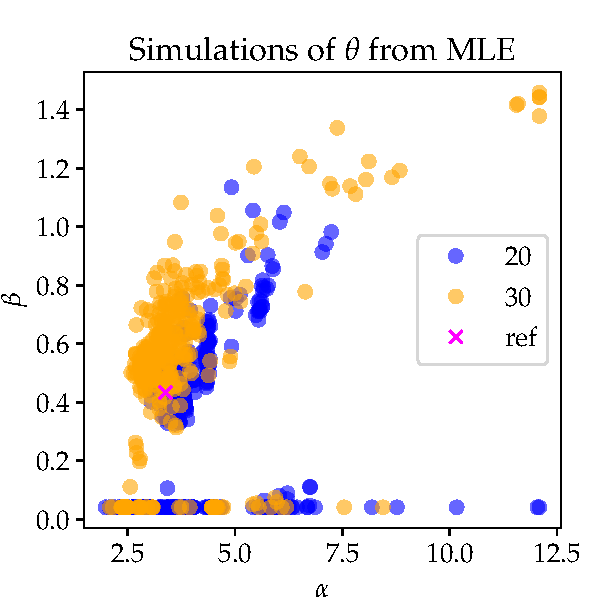
\includegraphics[width=130pt]{figures/MLE_scat_light.pdf}%
    %\hspace*{-0.1\linewidth}\includegraphics[width=1.2\linewidth]{figures/scatter.pdf}
     \caption{Scatter plots of the generated $\theta$ for the estimation of the fragility curves presented in \cref{fig:curvesONL} for the elasto-plastic oscillator. For all three statistical methods, we plotted $5000$  $\theta=(\alpha,\beta)$ {estimated} with two observed datasets of size $k=20$ (left figure) and $k=30$ (right figure). The cyan cross represents $\theta^{\mathrm{MLE}}$ derived from the $10^5$ samples composing the validation dataset.
     %This figure reveals both the outliers generated from the SK prior (center) and the irregularities characterized by null estimates of $\beta$ for the coupled MLE and bootstrap approach (right).
     }
    \label{fig:scatterONL}
\end{figure}

Since the SK prior is calibrated to look like the Jeffreys prior, \cref{fig:curvesONL} shows a strong similarity between the Bayesian estimations of the fragility curves obtained with these two priors. However, \cref{fig:scatterONL} shows that many outliers are obtained with the SK prior. These values explain why the credibility intervals of the fragility curves are larger with the SK prior when $k = 20$. This observation is supported theoretically by the calculation provided in \cref{sec:PREM:Jeffreys}. There is actually a better convergence of the Jeffreys prior toward $0$ when $\beta\to\infty$. This superior asymptotic behavior obviously results in posteriors that happen to assign a lower probability to outlier points (a phenomenon particularly noticeable when the data sample is small) as well as to the weight of the likelihood within the posterior.

For a better understanding of this phenomenon, we calculated the quantitative metrics defined in \cref{sec:PREM:metrics}. For any $k$ ranging from $15$ to $100$, we considered $m=200$ different draws of observations $(\mbf z^k_{(j)},\mbf a^{k}_{(j)})_{j=1}^m$ in order to derive the average values and $95\%$-confidence intervals of the metrics $\cE^{|\mbf z^k_{(j)},\mbf a^k_{(j)}}$, $\cW^{|\mbf z^k_{(j)},\mbf a^k_{(j)}}$, $j\in\{1,\dots,m\}$, for each of the three methods. %, $L=5000$, $1-r=95\%$. 
They are plotted in \cref{fig:errors}. Firstly, these diagrams demonstrate the benefits of the Bayesian framework compared to the MLE approach for small observation sets. Secondly, the compared performance of the Jeffreys and SK posteriors is highlighted by the confidence interval endpoints of the quadratic error and the credibility interval. Specifically, the latter highlights the effect of the superior asymptotic behavior of the Jeffreys prior along the width of the credibility interval. It shows variations similar to but smaller than the SK prior, thus highlighting its capacity to generate fewer outliers for the pair $(\alpha, \beta)$, as expected.

\begin{figure}[h]
    \centering%
    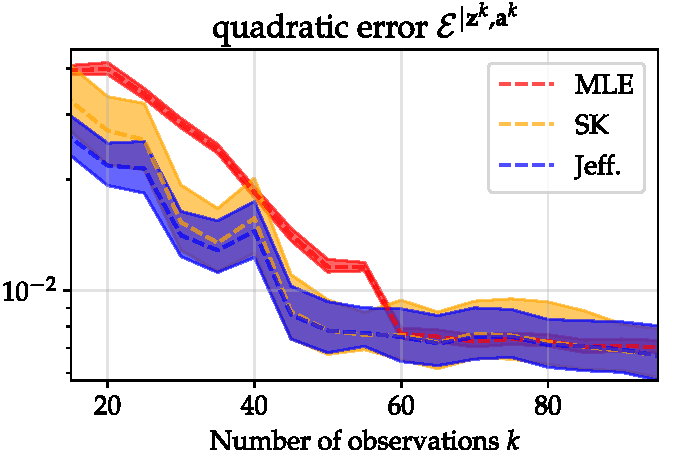
\includegraphics[width=5.2cm]{figures/PREM/oscill/errElog.pdf}\hspace*{0.5cm}
    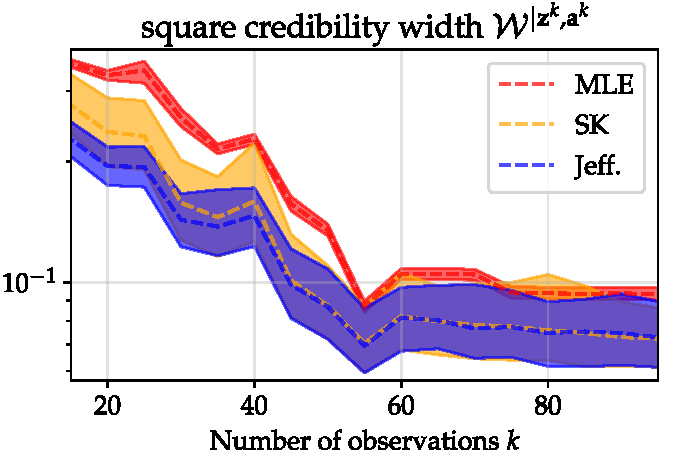
\includegraphics[width=5.2cm]{figures/PREM/oscill/errWlog.pdf}
    %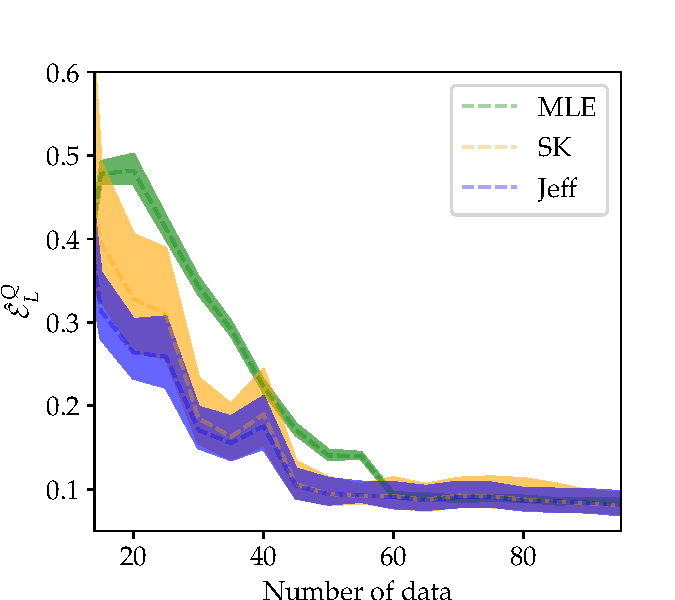
\includegraphics[width=154pt]{figures/erreur_quadratique.pdf} %0.4\linewidth
    % 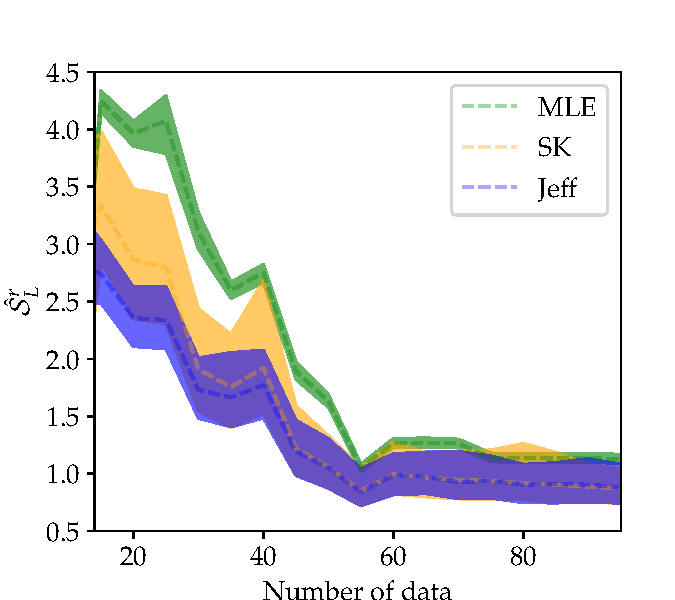
\includegraphics[width=154pt]{figures/taille_zone_credib.pdf}%
    \caption{%
    Average values of the performance evaluation metrics $\cE^{|\mbf z^k,\mbf a^k}$ (left) and $\cW^{|\mbf z^k,\mbf a^k}$ (right) for the elasto-plastic oscillator computed by replications of the experiment with different observation sets and for different sample sizes, ranging from $k=15$ to $100$. In each figure, the shaded areas show the $95\%$-confidence intervals of the metrics.}
    \label{fig:errors}
\end{figure}





\subsection{Case study 2: the piping system from a pressurized reactor}

% \textcolor{orange}{description}

This second case study deals with a piping system which is part of the secondary cooling system of a French pressurized water reactor. This piping system was presented in details in   \cref{chap:frags-intro} (\cref{sec:intro-frags:piping}).
% We evoked in   \cref{labellist}
Nonlinear dynamical simulations of this system's response have been carried out for $8\cdot10^4$ of the seismic signals we dispose.
The resulting validation dataset in the plan (PGA,EDP) is depicted in \cref{fig:PREM:asg}, along with a picture of the system's mock-up and reference fragility curves derived using non-parametric estimation from the validation set (as explicated in \cref{sec:PREM:metrics}).
In this study, the failure is defined when the EDP exceeds a threshold $C=3.8^\circ$.

%Along with a picture of the system's mock-up, the resulting validation 



%was studied experimentally and numerically within the framework of the ASG program \cite{TOUBOUL1999}

\begin{figure}[h]
    \centering
    \parbox[b][3.8cm][c]{4.5cm}{%
    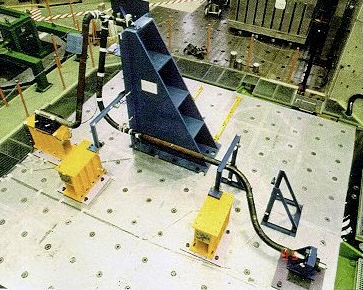
\includegraphics[height=3.2cm]{figures/intro-frags/ASG.jpg}\vspace*{1em}%
    }
    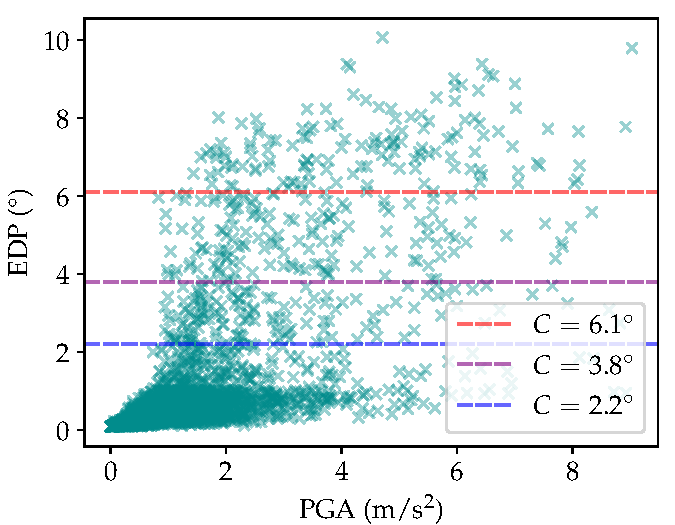
\includegraphics[height=3.8cm]{figures/intro-frags/asg/cloud_PGA_light.pdf}\ \ 
    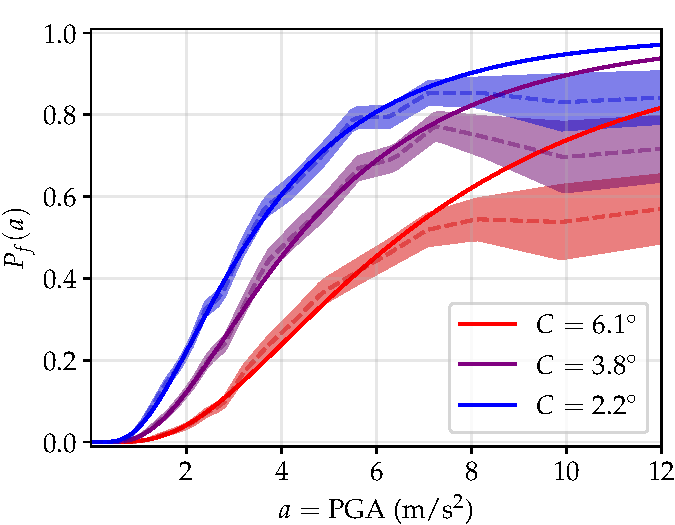
\includegraphics[height=3.8cm]{figures/intro-frags/asg/refs_PGA.pdf}
    \caption{Illustration of the second case study. Left: picture of the mock-up on the Azalee shaking table of CEA. Middle: results of $8\cdot10^4$ non-linear dynamical simulations. Right: reference non-parametric fragility curves (dashed lines) surrounded by their $95\%$-confidence intervals, compared with the probit-lognormal fragility curves derived by MLE from the validation dataset of size $8\cdot 10^4$. Different thresholds $C$ are considered, each yields different proportions of failures in the validation dataset: resp. $95\%$ (red), $90\%$ (purple) and $85\%$ (blue).}
    \label{fig:PREM:asg}
\end{figure}




Estimations similar to the first case study’s were performed here, and highlighted the same trends % were found to highlight the same trends.
As expected, for sets of $5000$ values of $\theta$ ---generated with each statistical method considered in this work--- and for two sample sizes $k = 20$ and $k = 30$ of nonlinear dynamical simulations, \cref{fig:ASG-curves} shows the superiority of the Bayesian framework over the coupled MLE and bootstrap approach. Just like in the case study with the oscillator, irregularities appear with the MLE-based approach: the confidence intervals are similarly ``quasi-vertical'', reflecting the fact that many estimations of $\beta$ are equal to $0$. Moreover, the credibility intervals are wider with the SK prior than with the Jeffreys prior, which here too can be interpreted as an increased number of outliers. % of $\theta$ being generated with the SK prior. 
These observations are clearly supported by the results presented in \cref{fig:ASG-scatter}.


\begin{figure}[h]
    \centering
    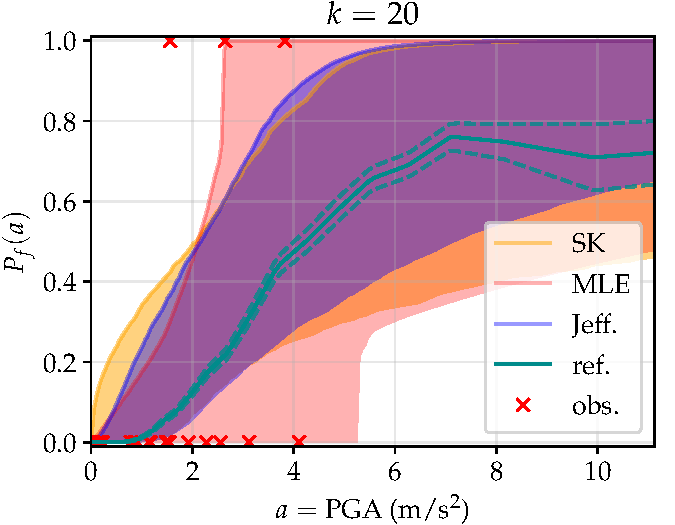
\includegraphics[width=5.2cm]{figures/PREM/asg/PGA20.pdf}\hspace*{0.5cm}
    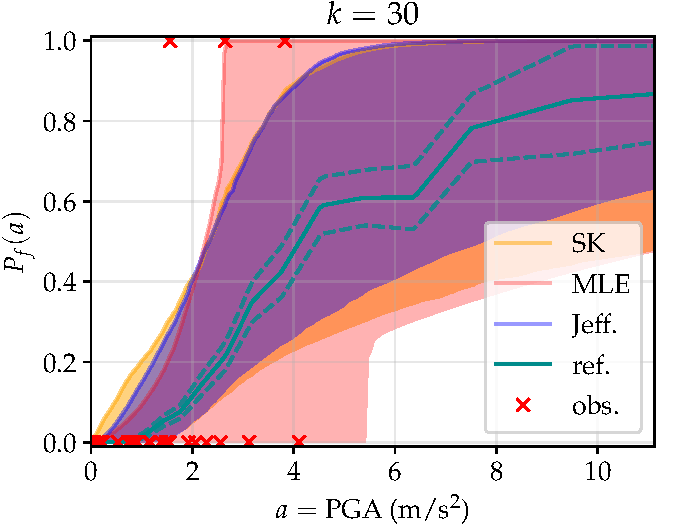
\includegraphics[width=5.2cm]{figures/PREM/asg/PGA30.pdf}
    % 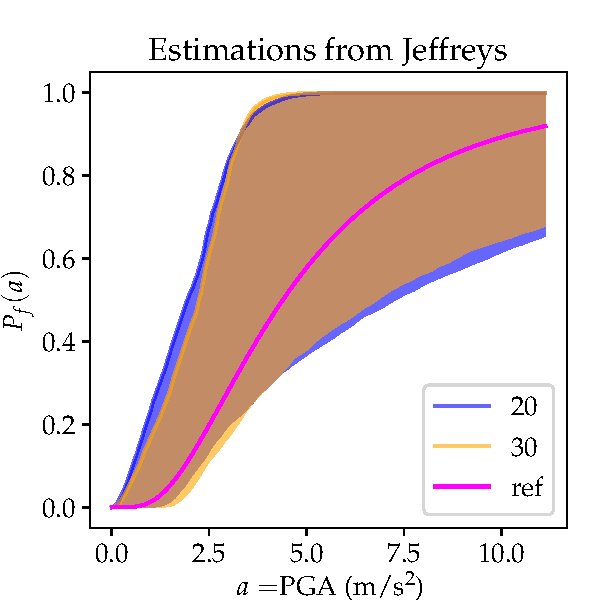
\includegraphics[width=130pt]{figures/curves_ASG_Jeff.pdf}%
    % 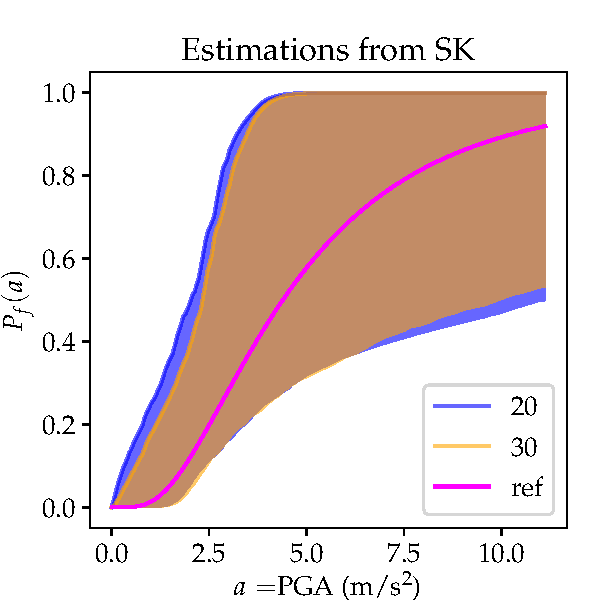
\includegraphics[width=130pt]{figures/curves_ASG_SK.pdf}%
    % 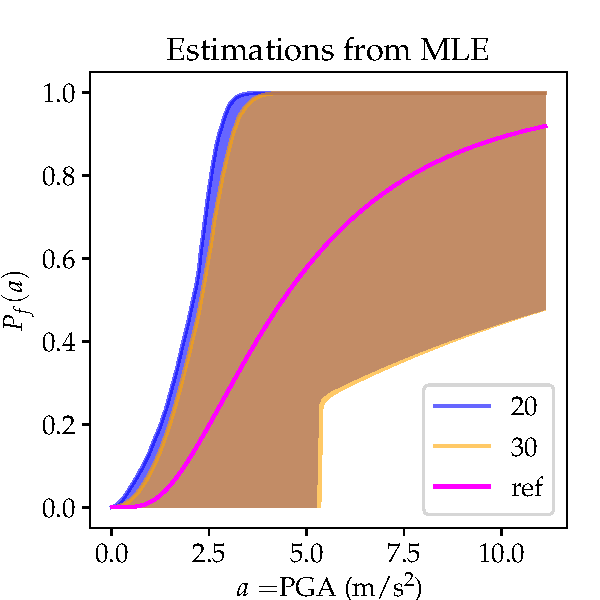
\includegraphics[width=130pt]{figures/curves_ASG_MLE.pdf}% 0.32\linewidth
    \caption{$95\%$ credibility (for Bayesian estimation) or confidence (for the MLE) intervals of fragility curve estimations for the piping system, using the methods described in \cref{sec:PREM:competing}. %, obtained from a total of $5000$ estimations of $\theta$ using the {statistical methods introduced in \cref{sec:PREM:metrics}. In the left (resp. right) figure $k=20$ (resp. $k=30$) data are observed. 
    The cyan curve is the reference $P^\text{ref}_f$ suggested in \cref{sec:PREM:metrics}, surrounded by its $95\%$-confidence interval (dashed lines). The red crosses represent the observed data.}
    %\caption{$95\%$ credibility (for Bayesian estimation) or confidence (for the MLE) intervals of fragility curve estimations for the piping system, obtained from a total of $L=5000$ estimations of $\theta$ using the {statistical methods introduced in Section~ {sec:reference}}: (from left to right) Bayesian estimation using the Jeffreys prior, Bayesian estimation using the SK prior, and MLE with bootstrapping. For each of these, we considered two data samples {of nonlinear dynamical simulations} of two different sizes ($k=20$ in blue, $k=30$ in orange). $P_f^{\mathrm{MLE}}$ (see Section~ {sec:metrics}) is plotted in magenta.}
    \label{fig:ASG-curves}
\end{figure}


\begin{figure}[h!]%
    \centering%
    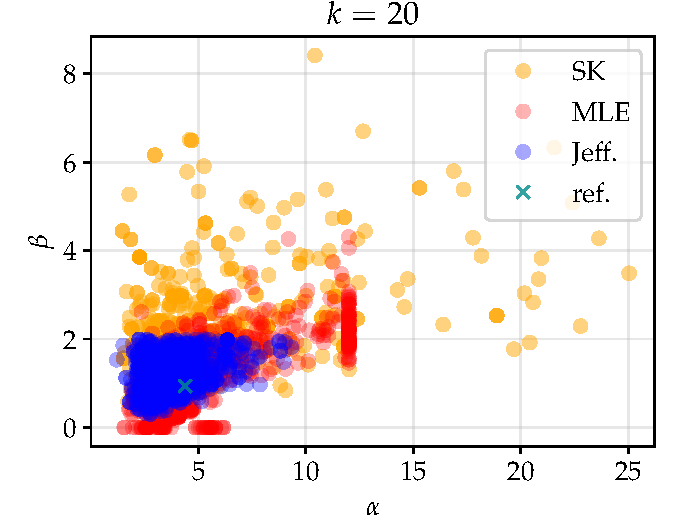
\includegraphics[width=5.2cm]{figures/PREM/asg/PGA20scatter.pdf}\hspace*{0.5cm}
    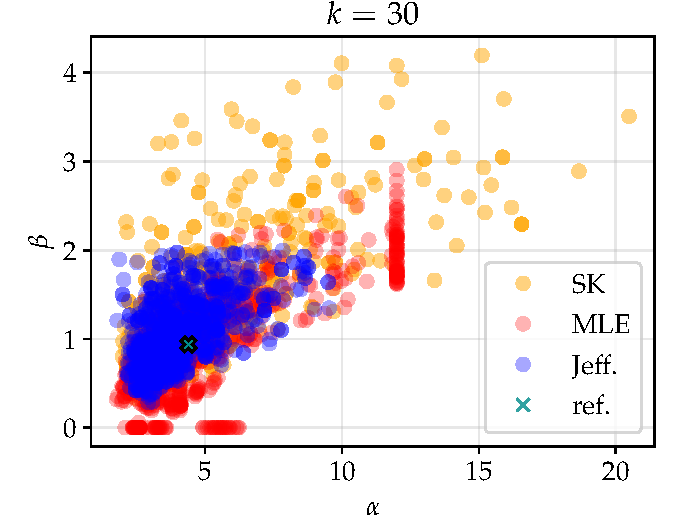
\includegraphics[width=5.2cm]{figures/PREM/asg/PGA30scatter.pdf}
    % 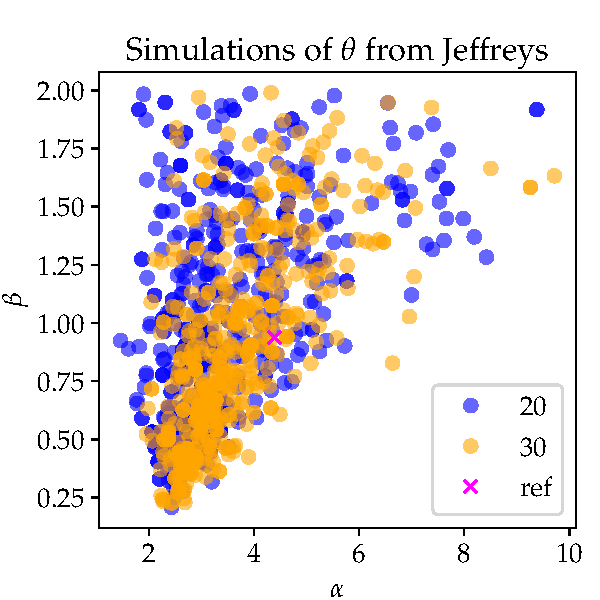
\includegraphics[width=130pt]{figures/scatter_ASG_Jeff_light.pdf}% 0.32\linewidth
    % 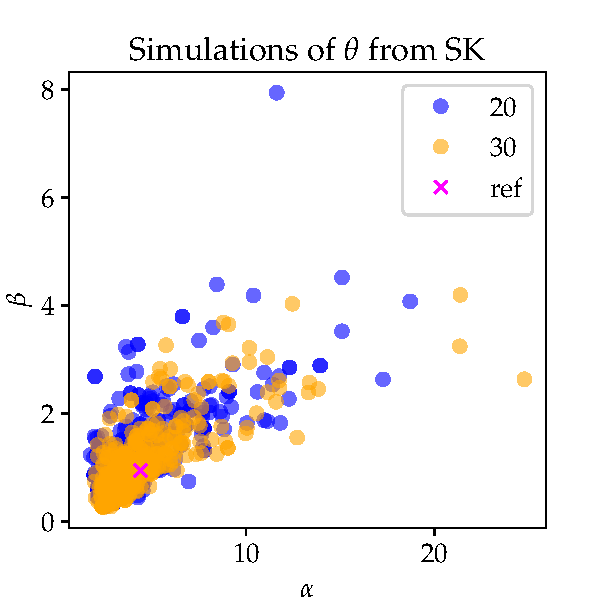
\includegraphics[width=130pt]{figures/scatter_ASG_SK_light.pdf}%
    % 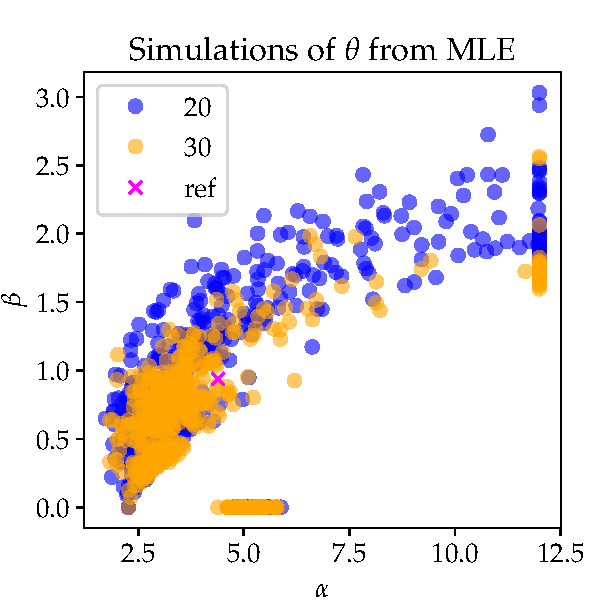
\includegraphics[width=130pt]{figures/scatter_ASG_MLE_light.pdf}%
    \caption{Scatter plots of the generated $\theta$ for the estimation of the fragility curves presented in \cref{fig:curvesONL} for the piping system. For all three statistical methods, we plotted $5000$  $\theta=(\alpha,\beta)$ {estimated} with two observed datasets of size $k=20$ (left figure) and $k=30$ (right figure). The cyan cross represents $\theta^{\mathrm{MLE}}$ derived from the $10^5$ samples composing the validation dataset.}
    %\caption{Scatter plots of the generated $\theta$ for the estimation of the fragility curves presented in Figure~ {fig:ASG-curves} for the piping system. For all three statistical methods, we plotted $500$ points out of the $L=5000$ $\theta=(\alpha,\beta)$ estimated with two data sets of nonlinear dynamical simulations (of size $k=20$ in blue and $k=30$ in orange). The magenta crosses represent $\theta^{\mathrm{MLE}}$, used for the computation of $P_f^{\mathrm{MLE}}$ {(see Section~ {sec:metrics})}. This figure unveils both the outliers generated from the SK prior (center) and the irregularities characterized by null estimates of $\beta$ for the coupled MLE and bootstrap approach (right).}
    \label{fig:ASG-scatter}
\end{figure}






For a more complete overview of their relative performances, the evaluation metrics described in \cref{sec:PREM:metrics}  have been computed in the same way as for the first case study: $m=200$ draws of data samples $(\mbf z^k_{(j)},\mbf a^k_{(j)})_{j=1}^m$ have been randomly chosen to compute, for any value of $k$ ranging from $15$ to $100$, the average values and $95\%$-confidence intervals of the metrics $\cE^{|\mbf z^k_{(j)},\mbf a^k_{(j)}}$, $\cW^{|\mbf z^k_{(j)},\mbf a^k_{(j)}}$, for each of the three methods. They are presented in \cref{fig:ASG-errors}. These results confirm the superior performance of the Jeffreys prior compared to the other two methods.    





\begin{figure}[h!]
    \centering%
    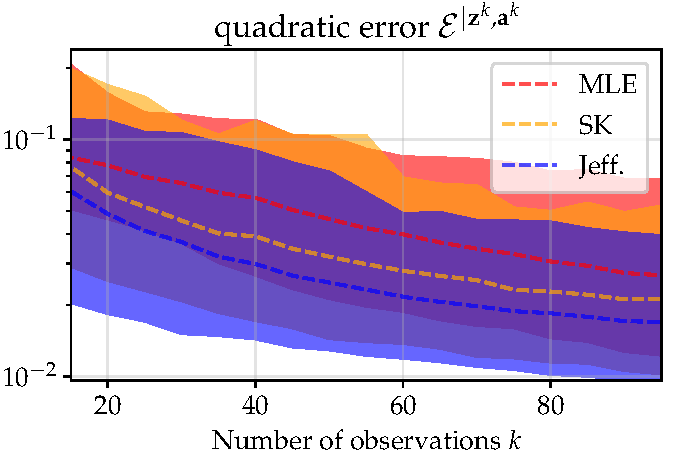
\includegraphics[width=5.2cm]{figures/PREM/asg/errElog.pdf}\hspace*{0.5cm}
    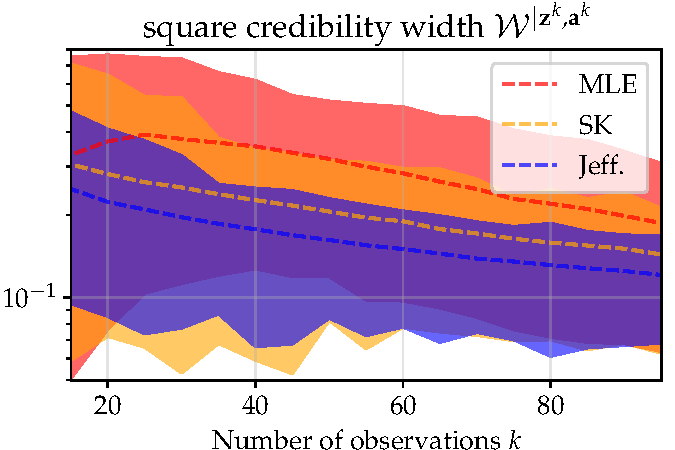
\includegraphics[width=5.2cm]{figures/PREM/asg/errWlog.pdf}
    %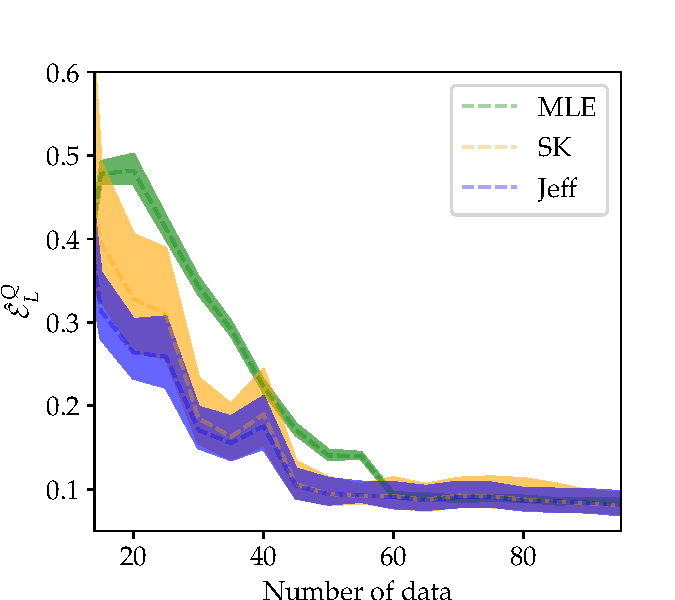
\includegraphics[width=154pt]{figures/erreur_quadratique.pdf} %0.4\linewidth
    % 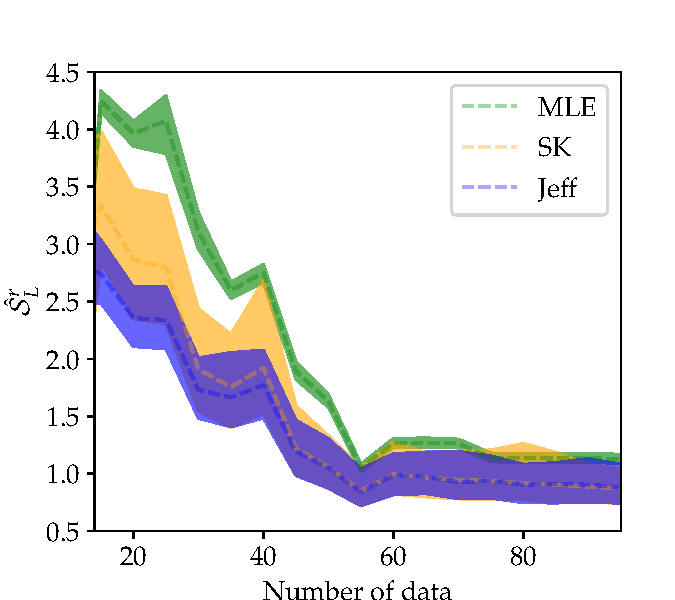
\includegraphics[width=154pt]{figures/taille_zone_credib.pdf}%
    \caption{%
    Average values of the performance evaluation metrics $\cE^{|\mbf z^k,\mbf a^k}$ (left) and $\cW^{|\mbf z^k,\mbf a^k}$ (right) for the piping system computed by replications of the experiment with different observation sets and for different sample sizes, ranging from $k=15$ to $100$. In each figure, the shaded areas show the $95\%$-confidence intervals of the metrics.}
    \label{fig:ASG-errors}
\end{figure}


% \begin{figure}
%     \centering%
%         % 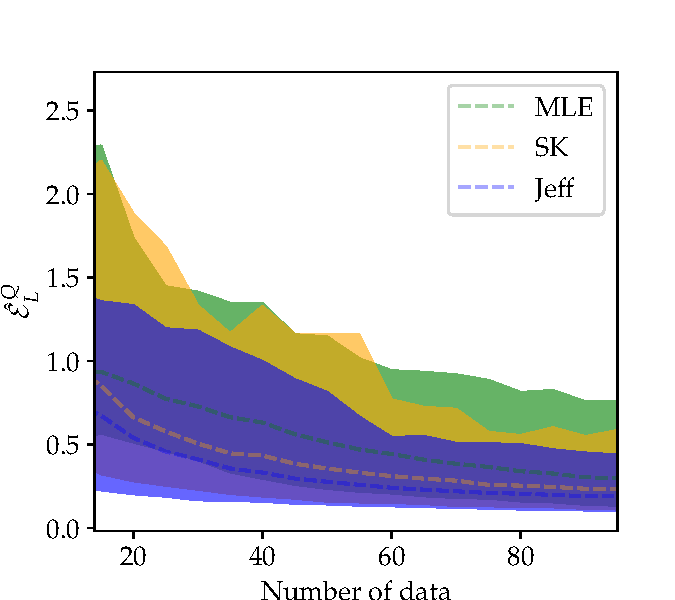
\includegraphics[width=154pt]{figures/ASG_quadra_error.pdf} %0.4\linewidth
%         % 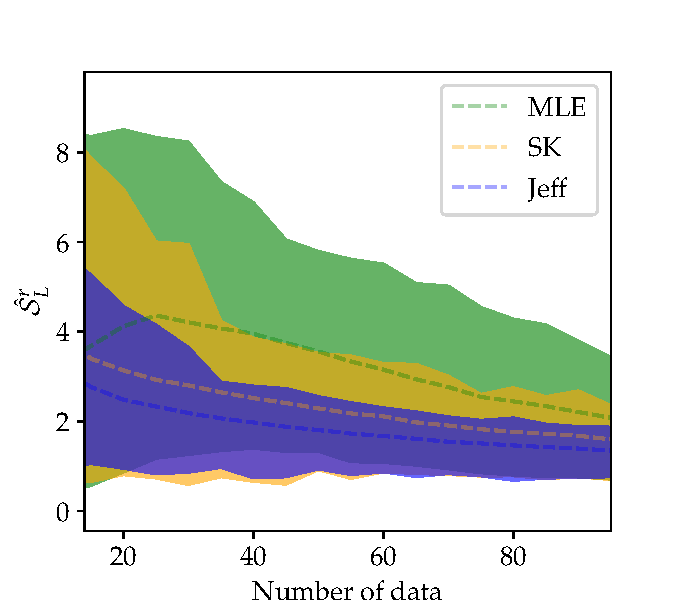
\includegraphics[width=154pt]{figures/ASG_cred_width.pdf}%
%         \caption{Performance evaluation metrics (see Section~ {sec:metrics}) for the piping system computed by replications from independent draws in the full data set of nonlinear dynamical simulations and for sample sizes ranging from $k=15$ to $100$. Left: the dashed lines plot the quadratic errors as a function of the number of observations, and the shaded areas show their confidence intervals. Right: the dashed lines plot the widths of the credibility intervals (for the Bayesian estimation) or confidence intervals (for the MLE), and the shaded areas show their confidence intervals.}
%     \label{fig:ASG-errors}
% \end{figure}






\subsection{Case study 3: the stacked structure for storage of packages}


The case study considered hereafter concerns a freestanding stacked structure composed of three pallets intended
for the storage of packages. A complete description of the system was proposed in   \cref{chap:frags-intro}. In \cref{fig:PREM:EDEN}-left. %, we 
% depict a picture of the structure and an example of test results.
%  and a picture of the structure is depicted in \cref{fig:PREM:EDEN}. 
%
%
%As shown in Figure 1, it is a square-based structure 3 meters high with a slenderness of
%2.4.
%
For this case study, only $k=21$
experimental results have been performed on a shaking table. %for seismic 
%fragility curve estimation. It illustrates the use of the
% method in practice and the interpretation of its results in a realistic context.
% This context does not permit the 
An example of a result is
shown in \cref{fig:PREM:EDEN}-right, which depicts the horizontal displacements over time of the top of the stack. The initial position is
indicated in red, while the different positions in time are indicated in blue. Due to uplift, sliding, and rotation motions,
the top of the stack exceeds, for 2 of the 21 tests, the admissibility criterion, which is materialized in black. Due to
the signals used for these tests, the Jeffreys prior is suitable for estimating a fragility curve of the stack, as is the SK
prior calibrated to approximate the Jeffreys prior.


\begin{figure}[h]
    \centering		
    \hspace*{0.3cm}\includegraphics[width=3cm]{figures/intro-frags/EDEN.jpg}
    \hspace{0.5cm}
    \includegraphics[width=6cm]{figures/intro-frags/EDEN_R169.pdf}
    \caption{(left) Overview of the stacked structure placed on the Vesuve 1D shaking table and (right) example of test result: horizontal displacements of the top of the stack when subjected to seismic excitation in the X direction.}
    \label{fig:PREM:EDEN}
\end{figure}  


The small number of data points does not allow comparison with a reference. Therefore, only a qualitative study can be carried out. \Cref{fig:PREM:eden-results} shows the results from $5000$ estimations of $\theta$ performed with the three {statistical methods considered in this study}. These results do not call into question the previous ones because they, once again, highlight the same phenomena, namely: (i) some irregularities of the MLE-based approach characterized by ``quasi-vertical'' confidence intervals; (ii) wider credibility intervals with the SK prior than with the Jeffreys prior; and (iii) the generation of many outliers of $\theta$ with the SK posterior compared to the Jeffreys posterior, which explains the slightly larger credibility intervals on the log-normal estimates of the fragility curves.

\begin{figure}[!h]
    \centering
    \includegraphics[width=5.2cm]{figures/PREM/EDEN/PGA21.pdf}\hspace*{0.5cm}
    \includegraphics[width=5.2cm]{figures/PREM/EDEN/PGA21scatter.pdf}
    \caption{Left: $95\%$ credibility (for Bayesian estimation) or confidence (for the MLE) intervals of fragility curve estimation for the stacked structure. The red crosses represent the observed data. Right: scatter plot of the $5000$ generated $\theta$ used for the computation of the credibility or confidence zones depicted in the left figure.}
    \label{fig:PREM:eden-results}
\end{figure}


\section{A review of the properties of the SK posterior}\label{app:SKreview}



In this chapter, we have compared our approach with the one that results from an adaptation of the prior suggested by \citet{straub_improved_2008}. We proved in \cref{sec:PREM:degeneracy} that within our framework, this prior results in an improper posterior. This puts the validity of the MCMC estimations into question, and could explain the lower performance of the SK prior compared to the Jeffreys prior. 
In their paper, the authors use the Bayesian methodology the same way we do, yet the consideration of uncertainties over the observed earthquake intensity measures and the equipment capacities leads to a slightly different likelihood.
In order to verify that the drawbacks of their prior highlighted in this chapter are not due to our statistical choices, we dedicated this section to the study of the asymptotic expansions of the posterior in the exact framework presented in \cite{straub_improved_2008}.
We shall first introduce the exact model of their paper for the estimation of seismic fragility curves in \cref{subapp:C1}, using notations consistent with our study. We will then derive the likelihood and its asymptotics in \cref{subapp:C2}. Finally, we will express the convergence rates of the posterior in \cref{subapp:C3}, which will allow us to conclude that the SK posterior is indeed improper.

\subsection{Statistical model and likelihood}
\label{subapp:C1}
Let us consider the observations of earthquakes labeled $l=1,\dots,L$ at equipment labeled $i=1,\dots,I_j$ located in substations labeled $j=1,\dots,J$.
The observed items are $(\mbf z_{jl},\hat a_{jl})_{j,l}$, $\mbf z_{jl}=(z_{ijl})_i$ being the failure occurrences of the $I_j$ pieces of equipment at substation $j$ during earthquake $l$ ($z_{ijl}\in\{0,1\}$), and $\hat a_{jl}$ being the observed IM at substation $j$ during earthquake $l$ ($\hat a_{jl}\in(0,+\infty)$).
They are assumed to follow the latent model presented below.

At substation $j$ the $l$-th earthquake results in an IM value $a_{jl}$ that is observed with an uncertainty multiplicative noise: $\log\hat a_{jl}=\log a_{jl}+\eps_{jl}$ where $\eps_{jl}\sim\cN(0,\sigma_\eps^2)$. The noise variance $\sigma_\eps^2$ is supposed to be known. %, and so $\sigma_\eps$ is considered known. % represents the estimation error.
The uncertain intrinsic capacity of equipment $i$ at substation $j$ is $r_{ij}\sim\cN(\mu_r,\sigma^2_r)$ and $y_{jl}\sim\cN(0,\sigma^2_y)$ is the uncertain factor common to all equipment capacities at substation $j$ during earthquake $l$.
The random variables $r_{ij}$, $y_{jl}$ and $\eps_{jl}$ are supposed to be independent.

A failure of equipment $i$ at substation $j$ during earthquake $l$ is considered when the performance of the structural component $g_{ijl}$ satisfies $g_{ijl}>0$.% for a certain threshold $C$. 
This performance can be expressed as 
    \begin{equation*}
      g_{ijl} = \log \hat a_{jl}+\eps_{jl}-y_{jl}-r_{ij}=x_{jl}-r_{ij}  
    \end{equation*}
with $x_{jl} = \log \hat a_{jl}+\eps_{jl}-y_{jl}$.
%Note that up to a change of the mean $\mu_r$, $C$ can be assumed to be equal to $0$. 

This establishes the following conditional relation between the observed data:
    \begin{equation}
        p(z_{ijl}|\hat a_{jl},\Sigma) =\hspace*{-3pt} \int_\RR p(z_{ijl}|x_{jl},\hat a_{jl},\Sigma)\frac{\exp\left({-\frac{(x_{jl}-\log\hat{a}_{jl})^2}{2(\sigma^2_\eps+\sigma^2_y)}}\right)}{\sqrt{2\pi(\sigma_\eps^2+\sigma_y^2)}}dx_{jl} ,
    \end{equation}
denoting $\Sigma=(\sigma_r,\,\sigma_y,\,\mu_r)$, and with 
    \begin{equation}\label{eq:SKr:condzx}
        p(z_{ijl}|x_{jl},\hat a_{jl},\Sigma) = \Phi\left(\frac{x_{jl}-\mu_r}{\sigma_r}\right)^{z_{ijl}}\left(1-\Phi\left(\frac{x_{jl}-\mu_r}{\sigma_r}\right)\right)^{1-z_{ijl}} \hspace*{-4pt} ,
    \end{equation}
when substation $j$ is only affected by one earthquake. The method proposed in \cite{straub_improved_2008} actually considers cases in which a substation may be impacted by two successive earthquakes and takes into account the fact that its response to the second would be correlated to its response to the first one. This would lead to a different likelihood. However, it is mentioned that this possibility only concerns a small number of data points. We can therefore limit our calculations to the simplest case and assume $l=L=1$. The subscript $l$ will therefore be dropped in what follows.

Finally, the likelihood for this model can be expressed as:
    \begin{equation}
    \label{eq:SKr:likelihood}
        \ell_J(\mbf z | \mbf{\hat a}, \Sigma)
            = \prod_{j=1}^J \int_\RR\prod_{i=1}^{I_j} p(z_{ij}|x_{j},\log\hat a_{j},\Sigma) \frac{\exp\left({-\frac{(x_{j}-\log\hat{a}_{j})^2}{2(\sigma^2_\eps+\sigma^2_y)}}\right)}{\sqrt{2\pi(\sigma_\eps^2+\sigma_y^2)}}dx_{j}  ,
    \end{equation}
denoting $\mbf z=(\mbf z_j)_{j=1}^J$, $\mbf{\hat a}=(\hat a_j)_{j=1}^J$, and with the integrated conditional distribution defined in \cref{eq:SKr:condzx}.


%\subsection{Prior}
    In the Bayesian framework introduced in \cite{straub_improved_2008}, the model parameter is $\Sigma$. Let us denote 
    $\alpha=\exp\mu_r$, $\beta=\sqrt{\sigma_r^2+\sigma^2_y}$ and $\rho=\sigma^2_y/\beta^2$. Denoting $\theta=(\alpha,\beta,\rho)$, the knowledge of $\Sigma$ then becomes equivalent to the one of $\theta$ and the likelihood of \cref{eq:SKr:likelihood} can be expressed conditionally to $\theta$ instead of $\Sigma$:

    \begin{equation}
    \label{eq:SKr:likelihood-theta}
        \ell_J(\mbf z | \mbf{\hat a}, \theta)
            = \prod_{j=1}^J  \int_\RR\prod_{i=1}^{I_j} %\Phi\left(\frac{x-\log\alpha}{\beta\sqrt{1-\rho}}\right)^{z_{ij}}\left(1-\Phi\left(\frac{x-\log\alpha}{ \beta\sqrt{1-\rho}}\right)\right)^{1-z_{ij}}\\
            \Psi^{z_{ij}}\left(\frac{x-\log\alpha}{\beta\sqrt{1-\rho}}\right)
                \frac{\exp\left({-\frac{(x-\log\hat{a}_{j})^2}{2(\sigma^2_\eps+\rho\beta^2)}}\right)}{\sqrt{2\pi(\sigma_\eps^2+\rho\beta^2)}}dx ,%\nonumber
    \end{equation}
    where the notation $\Psi^{z_{ij}}(\gamma)$ is used to denote $\Phi(\gamma)^{z_{ij}}(1-\Phi(\gamma))^{1-z_{ij}}$.

    %This parameter $\theta$ is considered as an r.v. which follows the improper prior distribution
    \citet{straub_improved_2008} propose the following improper prior distribution for the parameter $\theta$:
    \begin{equation}\label{eq:SKr:SKprior}
        \pi_{SK}(\theta) \propto \frac{1}{\beta\alpha}\exp\left(-\frac{(\log\alpha-\mu)^2}{2\sigma^2}\right)\indic_{0\leq\rho\leq1}.
    \end{equation}
    \emph{A posteriori} estimations of $\theta$ are consequently generated from MCMC methods % to sample of the posterior distribution
    \begin{equation}\label{eq:SKr:post}
        p(\theta|\mbf z,\mbf{\hat a})\propto \ell_J(\mbf z | \mbf{\hat a}, \theta)\pi_{SK}(\theta).
    \end{equation}
        
        
\subsection{Likelihood asymptotics}
\label{subapp:C2}
    In this subsection, we will study the asymptotics of the likelihood defined in \cref{eq:SKr:likelihood-theta} when $\beta\to\infty$.
    Let us first consider the substitution $u=(x-\log\hat a_j)/\sqrt{\sigma_\eps^2+\rho\beta^2}$ to express the likelihood as
    \begin{equation}
        \ell_J(\mbf z | \mbf{\hat a}, \theta) = \prod_{j=1}^J\int_\RR f_{j}^\beta(u)du,
        \quad\text{with}\quad
        f_{j}^\beta(u) = \prod_{i=1}^{I_j}\Phi(h_j^\beta(u))^{z_{ij}}(1-\Phi(h_j^\beta(u)))^{1-z_{ij}} \frac{e^{-\frac{u^2}{2}}}{\sqrt{2\pi}} ,
    \end{equation}
    with 
    \begin{equation}
        h_j^\beta(u) = \frac{(u+\log\hat a_j)\sqrt{\sigma_\eps^2+\rho\beta^2}-\log\alpha}{\beta\sqrt{1-\rho}}.
    \end{equation}
    This way, remembering that $0\leq\Phi(1-\Phi)\leq1$, an upper bound $u\mapsto e^{-u^2/2}/\sqrt{2\pi}$ can be found for $f_{j}^\beta$ for any $\beta,u$. It converges when $\beta \to +\infty$ as follows:
        \begin{equation}
            \lim_{\beta\rightarrow\infty} f_{j}^\beta(u)%\\
                = \prod_{i=1}^{I_J}%\Phi\left(\frac{(u+\hat a_j)\sqrt{\rho}}{\sqrt{1-\rho}}\right)^{z_ij}\left(1-\Phi\left(\frac{(u+\hat a_j)\sqrt{\rho}}{\sqrt{1-\rho}}\right)\right)^{1-z_{ij}}
                \Psi^{z_{ij}}\left(\frac{(u+\log\hat a_j)\sqrt{\rho}}{\sqrt{1-\rho}}\right)
                \frac{e^{-\frac{u^2}{2}}}{\sqrt{2\pi}}.
        \end{equation}
    This gives the following limit for the likelihood:
        \begin{equation}\label{eq:SKr:limitlik}
            \lim_{\beta\rightarrow\infty}\ell_J(\mbf z | \mbf{\hat a}, \theta)
                = \prod_{j=1}^J\int_\RR \prod_{i=1}^{I_j}%\Phi\left(\frac{(u+\hat a_j)\sqrt{\rho}}{\sqrt{1-\rho}}\right)^{z_ij}\left(1-\Phi\left(\frac{(u+\hat a_j)\sqrt{\rho}}{\sqrt{1-\rho}}\right)\right)^{1-z_{ij}}
                \Psi^{z_{ij}}\left(\frac{(u+\log\hat a_j)\sqrt{\rho}}{\sqrt{1-\rho}}\right)
                \frac{e^{-\frac{u^2}{2}}}{\sqrt{2\pi}}du ,
        \end{equation}
    which is a positive quantity.


    \subsection{Posterior asymptotics}
\label{subapp:C3}
    By combining \cref{eq:SKr:limitlik,eq:SKr:post,eq:SKr:SKprior} we obtain the posterior asymptotics
    \begin{equation}
            p(\theta|\mbf z, \mbf{\hat a}) \equi{\beta\rightarrow{\infty}} \frac{C}{\beta},
        \end{equation}
 with $C$ being a positive constant.
    This makes the posterior improper w.r.t. $\beta$, with the same convergence rate as the one derived in our framework.
        
    


\section{Conclusion}





Assessing the seismic fragility of SCs is a daunting task when data is limited. The performance of the Bayesian framework in this kind of situation is well-known. Nevertheless, choosing a prior remains difficult because its impact on the \emph{a posteriori} distribution cannot be neglected, and therefore neither can its impact on the estimation of any relevant element linked to the fragility curves. 

Elaborating on the reference prior theory in order to define an objective prior, we derived, for the first time in this field of study, the Jeffreys prior for the log-normal model, with binary data that indicates the state of the structure (i.e. failure or non-failure). This prior is completely defined and thoroughly studied, and does not depend on any additional subjective choice.

This work is also an opportunity to develop a better theoretical understanding of the conditions that result in irregular fragility curves such as  unit-step functions in practice. This issue is quite inevitable when data is limited, since such curves are a result of the very composition of the sample. Although this issue affects every approach, 
our results prove the robustness of the proposed approach over the traditional ones in terms of regularization (i.e. the absence of irregular estimation of the fragility curve) and stability (i.e. the absence of outliers when sampling the \emph{a posteriori} distribution of the parameters).  %is %outperform
%how that phenomenon affects priorly 
Nevertheless, we recall that the study conducted in the present chapter does not permit generating reliable estimate
when the
%present study is limited to the generation of estimates when the 
observed data yield what we call a degenerate likelihood. In the latter case, we have proven theoretically that all the methods carried out in this chapter ---including ours--- are jeopardized.
That statement paves the way for further works that could (i)~reinforce the prior construction to suppress its posteriors' weaknesses under degenerate likelihoods; and (ii)~study methods for reducing the probability of the existence of degenerate likelihoods. These perspectives motivated the works that are presented in the following chapters of this manuscript.

% works are conducted in the following chapters of this manuscript.
% an and the methods to reduce 
%enhance the data curation in order to reduce 

%we could demonstrate rigorously ---i.e., both theoretically and numerically--- the robustness and advantages of the proposed approach over the traditional ones found in the literature for estimating fragility curves in terms of regularization (i.e., the absence of degenerate functions when sampling fragility curves with the \emph{a posteriori} distribution) and stability (i.e., the absence of outliers when sampling the \emph{a posteriori} distribution of the parameters). {The Jeffreys prior therefore leads to more robust credibility intervals.} 

Although the numerical implementation of the Jeffreys prior is complex ---more so than a prior defined as the product of two classical distributions such as log-normal distributions, for instance--- it is not a major issue. As a matter of fact, since it depends solely on the distribution of the IM, the ``cost'' of the initial calculation would quickly be recovered on the scale of an industrial installation containing several SCs whose fragility curves must be estimated. {For example, compared to methodologies that aim to define a prior based on mechanical calculations for a given SC, the advantage of the Jeffreys prior lies in its generic nature. The fact that it can be applied to all SCs subjected to the same seismic scenario largely compensates for the implementation of mechanical studies dedicated to each relevant SC. Additionally, the methodology can be implemented with any relevant IM without creating additional complexity.}


\newpage
\thispagestyle{plain}












